%%%%%%%%%%%%%%%%%%%%%%%%%%%%%%%%%%%%%%%%%%%%%%%%%%%%%%%%%%%%%%%%%%%%%%%%%%%%%%%
% template.tex - version 0.9.1.1 (5/26/2011)
%
% This is a template file for the osudiss-2 class. See
% osudiss-2.pdf for documentation, and the GS material 
% for the requirements.
%
% Copy the following osudiss-2 files your latex path (or just the folder containing this file):
% osudiss-2.cls (v0.9.1)
% sa-draftwater.sty
%
% Then, to compile this file:
% latex template
% bibtex template
% latex template
% latex template
%
% (You can also use pdflatex if you prefer.)
%
%%%%%%%%%%%%%%%%%%%%%%%%%%%%%%%%%%%%%%%%%%%%%%%%%%%%%%%%%%%%%%%%%%%%%%%%%%%%%%%
\documentclass[11pt, double, phd]{osudiss-2} 
% The `11pt' option is unnecessary since it is the default

% `onehalf' sets the line spacing to one-and-a-half spacing instead of
% double spacing.

% The `phd' option is unnecessary since it is the default

% Remove `draft' option for final draft

%%%%%%%%%%%%%%%%%%%%%%%%% Packages %%%%%%%%%%%%%%%%%%%%%%%%%
% Load your favorite packages here
\usepackage{graphicx} % for importing images in figures - you definitely want this!
\usepackage{lipsum} % for fake latin text---you probably don't want this
\usepackage{verbatimbox}

% For instance... see osudiss-2.pdf for some suggestions, if you don't
% have a clue
\usepackage{bm} % for bold math---useful
\usepackage{booktabs} % for more professional tables
\usepackage[titletoc]{appendix}

%hyperref packages and options
\usepackage{bookmark} % helps booksmarks look better in PDF
%hypersetup option 'breaklinks' is reguired for line wrapping in the table of contents during latex compilation, and can be removed if you use pdflatex
\hypersetup{colorlinks=true,linkcolor=blue, breaklinks} %internal links in blue, citations in green
%\hypersetup{colorlinks=true,linkcolor=black, citecolor=black, breaklinks} %all links in black
\usepackage[all]{hypcap}

%Use of natbib is STRONGLY recommended to sort and compress your references within each citation
%With these options, natbib will convert i.e. [5,3,9,4] to [3-5, 9]
\usepackage[sort&compress]{natbib}

%required to have latex automatically generate subfigures (i.e. (a), (b) etc)
\usepackage{subfig}
\usepackage[export]{adjustbox}
\setcounter{lofdepth}{2}
\PassOptionsToPackage{obeyspaces}{url}
%\usepackage{hyperref}% http://ctan.org/pkg/hyperref

%load glossaries packages
\usepackage[acronym, section=chapter]{glossaries}
%\usepackage[xindy,acronym, section=chapter]{glossaries} - recommended if supported by your OS
\makeglossaries %required to actually make a glossary
%A list of common acronyms
%Only those used will be displayed, so you can just add to this list


\newacronym{hhg}{HHG}{High Harmonic Generation}











 %load list of acronyms contained in acronyms.tex

%The following commands can be used to help deal with "overfull hbox" issues
%See, for example, http://www.tex.ac.uk/cgi-bin/texfaq2html?label=overfull for details
%\pretolerance 1000
\setlength{\emergencystretch}{3em}
%\tolerance 1000

%%%%%%%%%%%%%%%%%%%%%%%%% Custom Commands/Environments %%%%%%%%%%%%%%%%%%%%%%%%%
% Put your favorite custom commands here
\newcommand{\fish}{\alpha} % some of my students call it the "fish" symbol

%Print list of abbreviations - use same font as List of Figures and List of Tables for the title, and same formatting in the table of contents.
% Argument #1 - title for list of abbreviations (i.e. List of Abbreviations)

\newcommand\PrintListofAbbreviations[1]{
\phantomsection
\addcontentsline{toc}{front}{\typesetColumnHeading{#1}}
\printglossary[type=\acronymtype,title={\protect {\typesetLevelTwo{#1}}}]
}


\newenvironment{chapabstract}{%
    \begin{center}%
      \bfseries Abstract
    \end{center}}%

% Below is an example of customizing the style of headings in your
% dissertation. See osudiss-2.pdf for more information.
%
% For example, if you simply must have uppercase titles:
%\renewcommand\typesetLevelOne[1]{{\Large\textbf{\MakeUppercase{#1}}\par}}
%\renewcommand\typesetLevelTwo[1]{{\Large\textbf{\MakeUppercase{#1}}}}
% Note the \par for \typesetLevelOne
%
% If you want the title to be bold and |\Large| instead of |\Huge|:
%\renewcommand\titleFont{\normalfont\Large\bfseries}

% Add words that TeX may not know how to hyphenate below. This can
% help prevent overfull hboxes. For example,
\hyphenation{eigen-state space-time} 

%%%%%%%%%%%%%%%%%%%%%%%%% Document Metadata %%%%%%%%%%%%%%%%%%%%%%%%%
\title{Application of Attosecond Techniques to Condensed Matter Systems}
\author{Gregory J. Smith}
\advisorname{Louis F. DiMauro}
\degree{Doctor of Philosophy} % Default value
\member{L. Robert Baker}
\member{Jay A. Gupta}
\member{Yuri V. Kovchegov}
\authordegrees{M.Sc.}
\graduationyear{2019}
\unit{Graduate Program in Physics} 

%%%%%%%%%%%%%%%%%%%%%%%%% Begin Document %%%%%%%%%%%%%%%%%%%%%%%%%
\begin{document}

\frontmatter

\begin{abstract}

design and construction of attosecond transient absorption beamline.

design and testing of a bright XUV source

initial transient absorption experiments in germanium

\end{abstract}

\dedication{Dedicated to ???} % Optional, and seriously not this lame
\begin{acknowledgments}

Lou DiMauro and Pierre Agostini - of course. say something up here about them and the group in general.

Thank you to the following people who have helped me throughout my scientific career:

\begin{itemize}
	\item Stephen Hageman - most work in this thesis was done in close collaboration with Steve. major components of beamline were designed solely by Steve, and he was there to help in nearly every single experiment. endless discussions on nearly every aspect of all experimental and design work.
	\item Andrew Piper for designing the OMRON vacuum control system, and attempting to implement interferometric stabilization on the TABLe.
	\item Dietrich Keissewetter for coding the Thorlabs/Newport motor interface and the homemade beamline pointing software. Also, thanks for helping with the initial design of the TABLe apparatus, helping to chase down vibrations and making subtle improvements to the apparatus.
	\item Kent Talbert for writing the entire LavVIEW software data collection suite.
	\item Antoine Camper for implementing the phase plate and phase gratings, as well as helping calibrate the photon spectrometer.
	\item Jakub Husek, Anthony Cirri, Somnath Biswas \& Prof. Robert Baker for many discussions pertaining to data collection, experimental design and sample considerations.
	\item Cristian Ott for designing the original ``cage and crank" vacuum flange manipulator, which we adapted to work with our photon spectrometer.
	\item Sierra O'Bryan for doing the initial optical design of the photon spectrometer.
	\item Yaguo Tang, Michael Chilcote, Michael Newburger, Jinson Xu \& Yutichai Mueanngern from OSU, Prof. S.K. Sundaram from Alfred University, Grant Johnson, Venkateshkumar (Venky) Prabhakaran, Le Wang \& Yingge Du from PNNL - for sample preparation.
	\item Eric Moore for automating the TABLe alignment system.
	\item Marieke Jager from the Leone group and Norman Niewrzella from the Semiconductor Manufacturing Technology Business Group at Carl Zeiss SMT GmbH, for answering my questions about ellipsoidal mirrors.
	\item Pete Gosser and Michael Graham at the Physics Machine Shop for machining countless parts (including our vacuum chambers) and providing endless consulting about general machining practices. Special thanks to Jon Shover from the Astronomy Machine Shop for welding our vacuum chambers and some components on the high pressure cell.
	\item Tim Gorman for endless discussions about physics, experimental design, laser troubleshooting, and good conversations.
	\item Rich Pfisterer, Ryan Irvin and Donna Pfisterer from Photon Engineering, for providing me a university gratis software license of FRED, and for teaching me to use the software efficiently.
	\item Phil Davids and Mark Reed for helping out with general building problems. Kent Ludwig for helping repair our rough vacuum system.
	\item Kris Dunlap, Mary Kay Jackson, Shirley McClung, Dameyon Shipley, Kyle Schechter and Jessica Middleton for help with administrative issues.
	\item Jack Simonson, Carlos Marques, Meigan Aronson \& Jacob Grosse from BNL for fostering my interest in science and encouraging me to go to graduate school. They set me down this path and I thank them for it.
	\item From my time in Dr. Yang's group: Nick Minutillo, Yi-Shin Chiu, Zeke, Prof. Yang.
	\item Everyone else in the DiMauro group who has helped me throughout the years: Stephen Schoun, Tim Scarborough, Cosmin Blaga, Hyunwook Park, Junliang Xu, Urszula Szafruga, Kaikai Zhang, Kevin Gudenkauf, Zhou Wang, Yu Hang (Marco) Lai, Bryan Smith, Sha (Lisa) Li, Abraham Camacho, Daniel Tuthill, Vyacheslav (Slava) Leshchenko, Li Fang.
\end{itemize}


\end{acknowledgments}
\begin{vita}
\dateitem{Oct 17, 1990}{Born---Kolkata, India}
\dateitem{May, 2013}{B.S., NC State University, Raleigh, NC}
\dateitem{Dec, 2015}{M.S., Ohio State University, Columbus, OH}
% Insert other relevant items here (GTA, etc.)

\begin{publist}

\pubitem{``Constraints on the Diffuse High-Energy Neutrino Flux from the Third Flight of ANITA", 
P. W. Gorham, P. Allison, {\bf O. Banerjee} {\it et al.}, Physical Review D. 
I am a lead author and contributor of the new binned analysis presented, 
which is one of the three complementary analyses in the paper.
\href{https://arxiv.org/abs/1803.02719}{Link to electronic version.}}

\pubitem{``Dynamic tunable notch filters for the Antarctic Impulsive Transient Antenna (ANITA)'',
P. Allison, {\bf O. Banerjee} {\it et al.}, Nuclear Instruments and Methods A. 
I led this paper and served as {\bf corresponding author}. 
This paper is on the filters that I played a lead role in commissioning for ANITA-4, that helped to triple the livetime of the experiment.
%This is the first paper to describe the trigger systems of ANITA-3 and ANITA-4. 
\href{https://www.sciencedirect.com/science/article/pii/S016890021830411X}{Link to electronic version.}} 

I am also a co-author on all ANITA publications (6 total) since Jan 2016.

%\item ``Secret paper", A. Connolly, P. Allison, {\bf O. Banerjee}, Submitting to Astroparticle Physics. 
%This is a theoretical paper, and I worked closely with Connolly on literature review and simulation. 

%\item "GRB paper", O. Banerjee {\it et al.}, In progress for Astroparticle Physics. 

%\item ``Characteristics of Four Upward-pointing Cosmic-ray-like Events Observed with ANITA'',
%P. W. Gorham {\it et al.}, Phys.Rev.Lett. 117 (2016) no.7, 071101. I wrote a preliminary Monte Carlo simulation for energy loss of the tau lepton in different media. 

%\item ``Antarctic Surface Reflectivity Measurements from the ANITA-3 and HiCal-1 Experiments",
%P. W. Gorham {\it et al.}, J. Astron. Instrum. 06, 1740002 (2017). I gave comments. 

\end{publist}


\begin{fieldsstudy}
\majorfield{Physics}
\onestudy{Particle Astrophysics}{Connolly group} % optional
% Alternatively you can do:
\end{fieldsstudy}

\end{vita}

\tableofcontents 

% list of figures (comment out if you don't have any figures)
\clearpage %remove if you don't want a page break before list of figures
\listoffigures 

% list of tables (comment out if you don't have any tables)
%\clearpage  %remove if you don't want a page break before list of tables
%\listoftables 

%print glossary - comment out if you don't want this.  Make sure you also add \glsdisablehyper if you don't want to print a glossary, but do use the %glossaries package to keep track of acronyms
\clearpage %remove if you don't want a page break before list of abbreviations
\PrintListofAbbreviations{List of Abbreviations} %Title is in { } - change if desired
%\printglossary[type=\acronymtype]

\mainmatter
\chapter{Introduction}

\section{Ultrafast Dynamics in Condensed Matter Systems}

timescales and processes in solids

\section{Attosecond Transient Absorption Spectroscopy (ATAS)}

\subsubsection{why are you doing it with HHG?}

include figure of pulse duration vs photon energy, showing different light sources (synchrotrons, HHG sources, XFEL, etc.) tie this into the timescales neccessary to probe condensed matter physics.

\subsection{overview of the technique}

references \cite{ramaseshaRealTimeProbingElectron2016}

The basic concept of an \textit{attosecond transient absorption spectroscopy} (ATAS) experiment is shown in \cref{fig:ATAS_Cartoon_Si_Leone}. In this experiment, a sample is placed at the combined XUV/IR focus in a transmission (normal) geometry. An XUV photon spectrometer is placed behind the sample and the transmitted XUV spectrum $S$ is measured as a function of XUV-IR delay. The IR light is not measured by the spectrometer.

Fundamentally, changes in photoabsorption correspond to electron and phonon dynamics in the sample. In condensed matter materials, these processes occur on the picosecond ($10^{-12}$ s), femtosecond ($10^{-15}$ s) and even attosecond ($10^{-18}$ s) time scales \cite{schultzeAttosecondBandgapDynamics2014,cushingDifferentiatingPhotoexcitedCarrier2019,zurchDirectSimultaneousObservation2017,volkovAttosecondScreeningDynamics2019}. At XUV energies, photons drive electronic transitions from a core-level state to one near the Fermi level, which requires electron population in the initial state and a vacancy in the final state. Because the initial state is tens or even hundreds of eV below the bandgap, it is shielded from the external IR field. The final states, being closer to the Fermi level, enjoy no such shielding. Therefore they can be distorted by the external IR field, and the electron population can be transferred between these states in response to the IR field. After an initial IR excitation, electrons relax via different scattering channels, including with other electrons or phonon modes with longer lifetimes. Provided the dipole selection rules allow it, the photoabsorption spectrum is sensitive to all of these dynamics. Thus by measuring the XUV spectrum as a function of XUV-IR delay, we can track the electronic and phononic response of a sample to an ultrafast IR excitation.


\subsubsection{induced dipole interpretation}

\subsubsection{population transfer and probing interpretation}

\subsubsection{comparison of absorptive and reflective measurements}


\begin{figure}
	\centering
	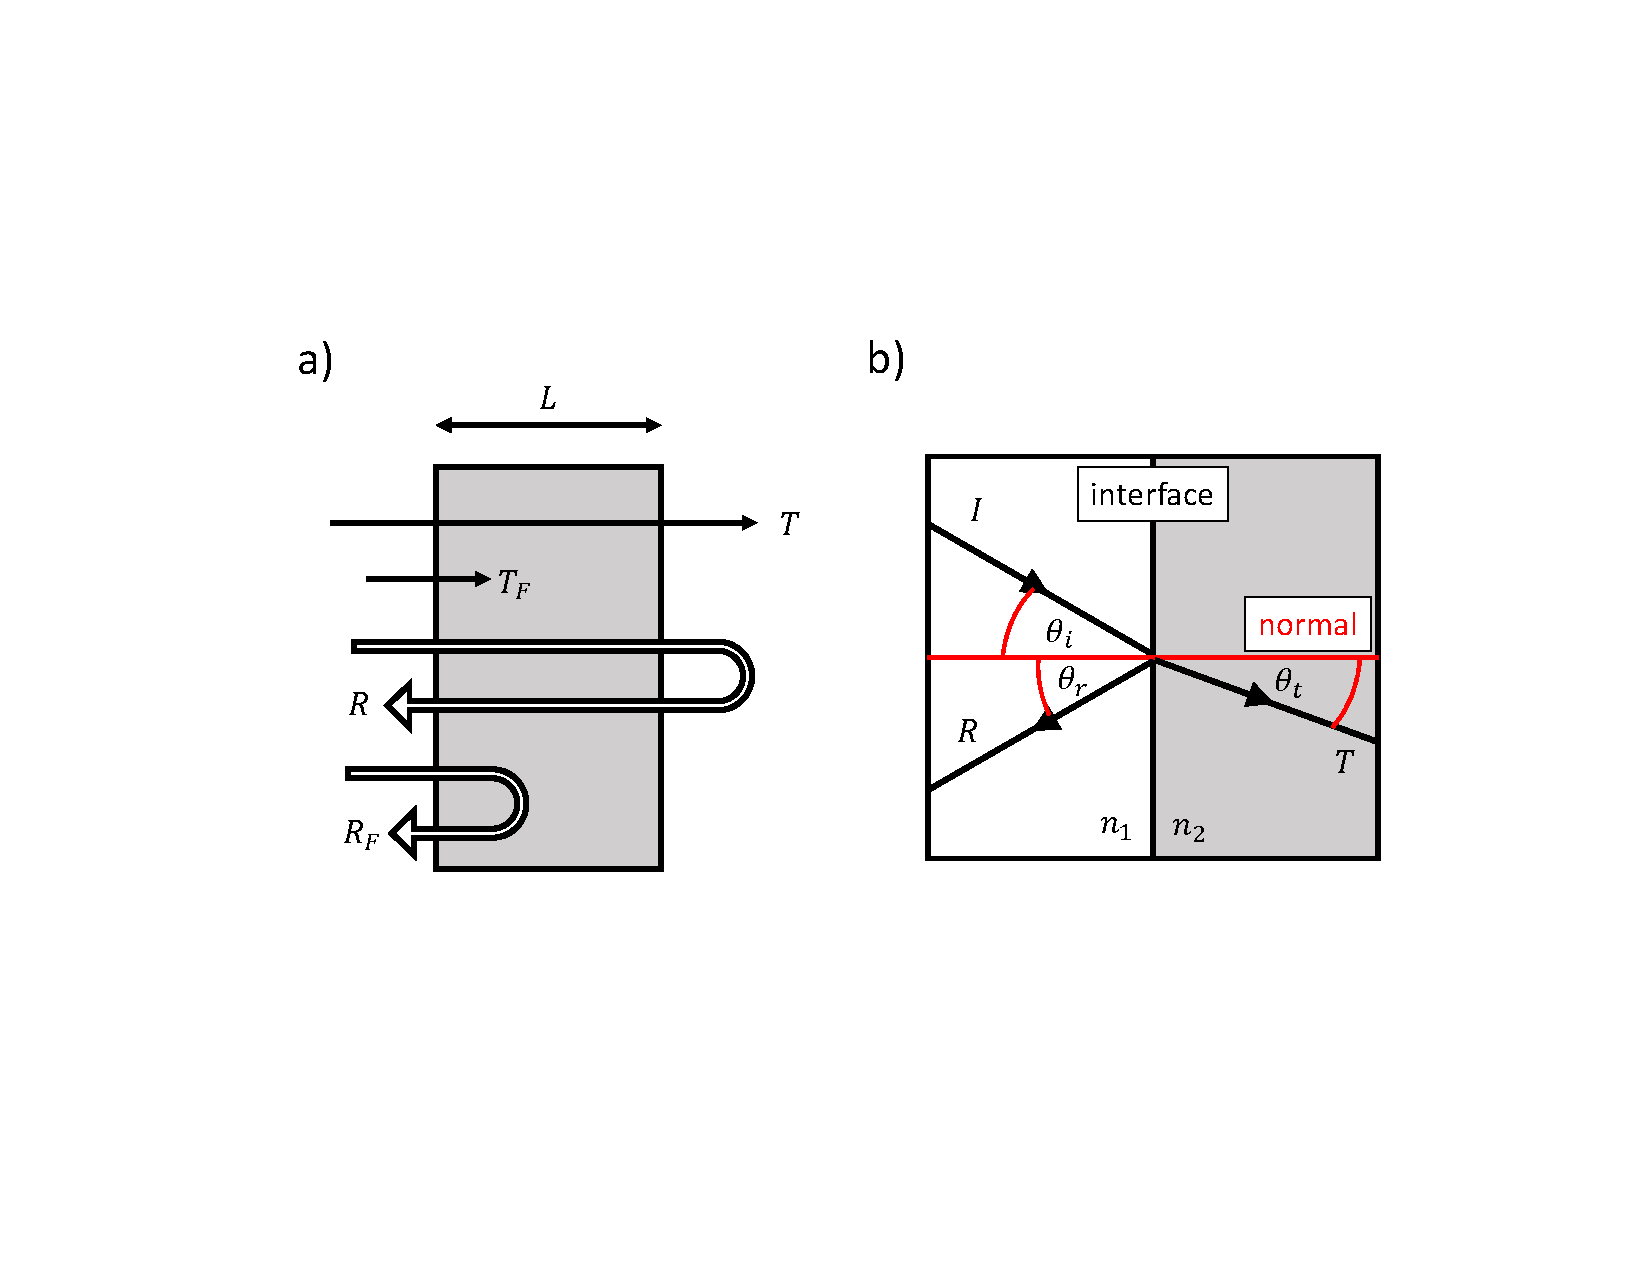
\includegraphics[width=0.75\textwidth]{figures/chap1/Fresnel_Geometry.pdf}
	\caption{Normal and non-normal incident geometries. \textbf{a)} Normal incidence geometry showing Fresnel coefficients $R_F$, $T_F$ for interfaces and total transmission $T$ and reflectance $R$ for a slab of thickness $L$. Figure recreated from \cite{nichelattiComplexRefractiveIndex2002}. \textbf{b)} Non-normal geometry showing definitions of angles $\theta_i, \theta_r$ and $\theta_t$ with respect to each interface.}
	\label{fig:Fresnel_Geometry}
\end{figure}

\begin{figure}
	\centering
	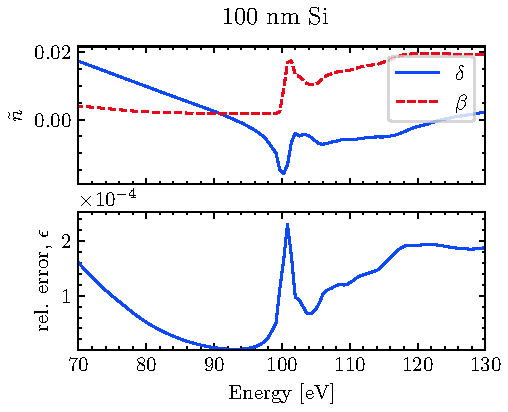
\includegraphics[width=0.75\textwidth]{figures/chap1/Si_transmission_Fresnel.pdf}
	\caption{Consequences of ignoring the real part of $\tilde{n}$ when calculating the transmission $T$ of a thin sample. Top panel: complex refractive index of silicon using the notation from \cref{eqn:complex_index}. The Si $L$-edge absorption feature is visible near 100 eV. Data from \cite{gulliksonCXROXRayInteractions}. Bottom panel: relative error in $T$, as defined in \cref{eqn:Fresnel_rel_err}, introduced by ignoring the contribution of $\Re(\tilde{n})$. An infinite number of bounces (e.g., \cref{eqn:Fresnel_coefs_inf_bounce}) is assumed.}
	\label{fig:Si_transmission_Fresnel}
	% plotted using \Python Scripts\CXRO\test\real_imag_index_plotting.py
\end{figure}

In a transient absorption experiment, we measure the transmission $T$ of a sample in response to excitation by an external field. Generally speaking, $T$ depends on both parts of the complex refractive index: $\tilde{n} = n + i k$. However, in a normal transmission geometry it turns out that the contribution of $\Im(\tilde{n})$ dominates the measured signal, and to a good approximation the role of $\Re(\tilde{n})$ can be ignored. Note that in a non-normal reflection geometry, both parts of $\tilde{n}$ make significant contributitions to the measured signal. In the following discussion we will analyze the Fresnel equations to see why this is the case. This section will draw from arguments made in reference \cite{nichelattiComplexRefractiveIndex2002}.

First, we consider the normal geometry shown in the left panel of \cref{fig:Fresnel_Geometry}. We write the complex index of refraction in the following form:
\begin{equation}
\begin{aligned}
\tilde{n} &= n - i k \\
&= (1-\delta) - i \beta
\end{aligned}
\label{eqn:complex_index}
\end{equation}
The Fresnel coefficients $R_F$ and $T_F$ describe the interface reflectance and transmittance and depend on both parts of the complex index $\tilde{n}$. For normal incidence, they are:
\begin{equation}
\begin{aligned}
R_F &= \left| \frac{n-ik-1}{n-ik+1}   \right|^2 \\
T_F &=  \frac{4n}{\left|n-ik+1\right|^2}
\end{aligned}
\label{eqn:fresnel_normal}
\end{equation}
Absorption in the bulk is described via the absorption length $\alpha$:
\begin{equation}
\alpha = 4 \pi k / \lambda
\end{equation}
Ignoring interface effects, the transmisison through the bulk is:
\begin{equation}
T_{\text{bulk}} = \exp( - \alpha L)
\end{equation}
Note that $\alpha$ and $T_{\text{bulk}}$ only depend on $k$.

The total reflectance $R$ and transmission $T$ are the result of interface effects plus bulk effects. We must consider the case where the detected light is the result of multiple reflections within the sample. Neglecting interference, we consider the case of $2N$ bounces where the laser's coherence length is less than the thickness of the bulk. In this case, the sum is incoherent with the expressions for $T$ and $R$ given by:
\begin{equation}
\begin{aligned}
R &= R_F + R_F T_F^2 T_{\text{bulk}}^2 \sum_{m=0}^{N} \left[ R_F T_{\text{bulk}} \right]^{2m} \\
T &= T_F^2 T_{\text{bulk}} \sum_{m=0}^{N} \left[ R_F T_{\text{bulk}} \right]^{2m}
\end{aligned}
\label{eqn:Fresnel_coefs_N_bounce}
\end{equation}
For the case of an infinite number of bounces, \cref{eqn:Fresnel_coefs_N_bounce} simplifies to:
\begin{equation}
\begin{aligned}
R &= R_F + \frac{R_F T_F^2 T_{\text{bulk}}^2}{1-R_F^2 T_{\text{bulk}}^2} \\
T &= \frac{T_F^2 T_{\text{bulk}}}{1-R_F^2 T_{\text{bulk}}^2},
\end{aligned}
\label{eqn:Fresnel_coefs_inf_bounce}
\end{equation}
whereas if only a single bounce occurs, \cref{eqn:Fresnel_coefs_N_bounce} reduces to:
\begin{equation}
\begin{aligned}
R &= R_F + R_F T_F^2 T_{\text{bulk}}^2 \\
T &= T_F^2 T_{\text{bulk}}
\end{aligned}
\label{eqn:Fresnel_coefs_1_bounce}
\end{equation}

We now consider the fractional error introduced by ignoring the interface effects described by $T_F$ and $R_F$. That is, what would happen if we assume that the interfaces have no effect on the transmitted intensity? We introduce the relative error $\epsilon$ made by ignoring the Fresnel coefficients of \cref{eqn:Fresnel_coefs_inf_bounce}:
\begin{equation}
\epsilon \equiv \frac{T_{\text{bulk}}}{T} - 1
\label{eqn:Fresnel_rel_err}
\end{equation}

As an example, consider a 100 nm thick Si sample measured in transmission near the Si $L$-edge (about 100 eV), as shown in \cref{fig:Si_transmission_Fresnel}. The relative error is in the range of one part in $10^4$ to $10^5$, well below our experimental detection limit. Silicon was chosen due to its data availability above and below the absorption edge, but this behavior should hold for all materials in normal transmission.

The real part of the complex index becomes important when the sample isn't normal to the beam, as shown in the right panel of \cref{fig:Fresnel_Geometry}. In this case, the Fresnel equations are a bit messier:
\begin{equation}
\begin{aligned}
R_s &= \left| \frac{\tilde{n}_1 \cos \theta_i - \tilde{n}_2 \cos \theta_t}{\tilde{n}_1 \cos \theta_i + \tilde{n}_2 \cos \theta_t}  \right|^2 \\
R_p &= \left| \frac{\tilde{n}_1 \cos \theta_t - \tilde{n}_2 \cos \theta_i}{\tilde{n}_1 \cos \theta_t + \tilde{n}_2 \cos \theta_i}  \right|^2 \\
T_s &= 1 - R_s \\
T_p &= 1 - R_p \\
%\theta_t &= \sqrt{1- \left( \frac{n_1}{n_2} \sin \theta_i \right)^2}
\end{aligned}
\label{eqn:Fresnel_nonnormal}
\end{equation}

Here, the subscripts $s$ and $p$ denote the polarization relative to the surface normal. For a sample in vacuum, $\tilde{n}_1=1$ and $\tilde{n}_2$ is the index of the sample. We can extract the relevant physics without any additional manipulation of \cref{eqn:Fresnel_nonnormal}. Right away, we can see that unlike \cref{eqn:fresnel_normal}, \cref{eqn:Fresnel_nonnormal} is symmetric in the real and imaginary parts of the sample's complex index, $\tilde{n}_2$. In the limit of a thick slab, ($L \gg \alpha$), the light is attenuated before it can reflect off the back surface and we have $T \rightarrow 0$ and $R \rightarrow R_{s,p}$. That is, the only contributions to the reflected intensity are from the interface and possibly the sample volume within $z \approx 1/\alpha$ of the interface. As a result, both parts of $\tilde{n}_2$ will make significant contributions to the reflected intensity. This geometry is common in transient reflection-absorption experiments \cite{cirriAchievingSurfaceSensitivity2017,kaplanFemtosecondTrackingCarrier2018}.



complex refractive index

sample requirements and preparation

pointing stability (in reflection, sample is an XUV optic)

\subsection{previous work}
what is state of the art?

previous work in condensed matter (Si, Ge, Si-Ge, etc)

motivation for long-wavelength studies in condensed matter

\subsection{physical observables in ATAS}
limited k-space information (requires single crystal)

transmission geometry measures imaginary and not the real part of n

\subsection{interpretation of experimental data}

\section{High Harmonic Generation}

High harmonic generation (HHG) is the extremely nonlinear process in which a strong infrared field produces light with frequencies that are integer multiples of the fundamental field after interacting with a medium. Rather than providing a first principles discussion of HHG, the main objective of this section is to understand how we can produce bright attosecond XUV light pulses with a sufficient spectral coverage for use in an ATAS experiment.

- spectral coverage of harmonics

- pulse duration of harmonic light

Gas phase HHG 

symmetry leads to odd harmonics.

gas and solid HHG has been studied

\subsection{Single Atom Response}

\begin{figure}
	\centering
	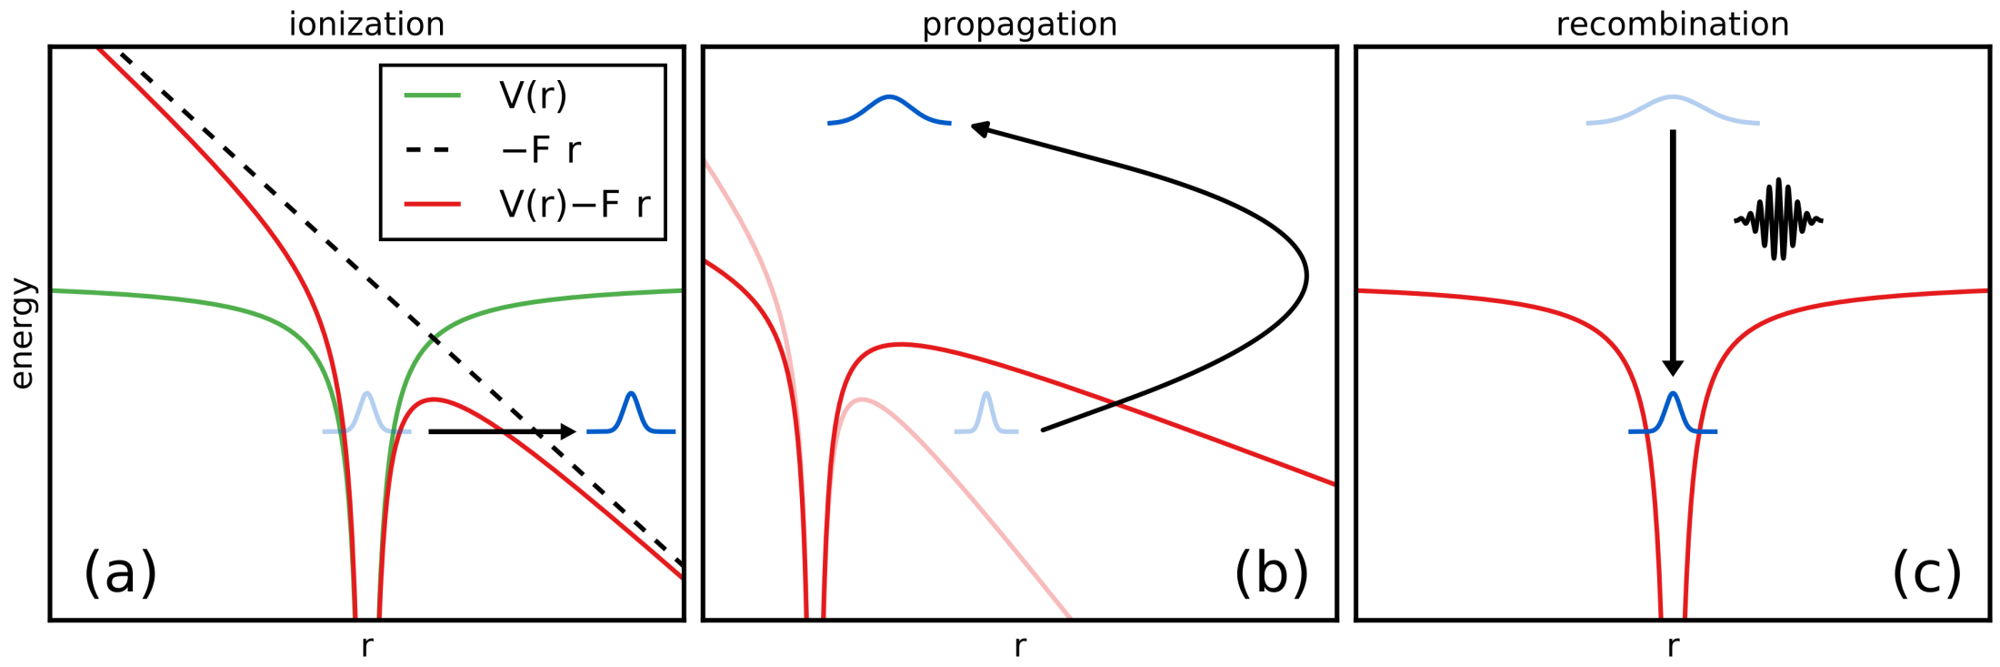
\includegraphics[width=0.75\textwidth]{figures/chap1/ThreeStepModel.png}
	\caption{The three step model of HHG. Figure adapted from \cite{schounAttosecondHighHarmonicSpectroscopy2015}.}
	\label{fig:ThreeStepModel}
\end{figure}

\begin{figure}
	\centering
	\subfloat[]{
		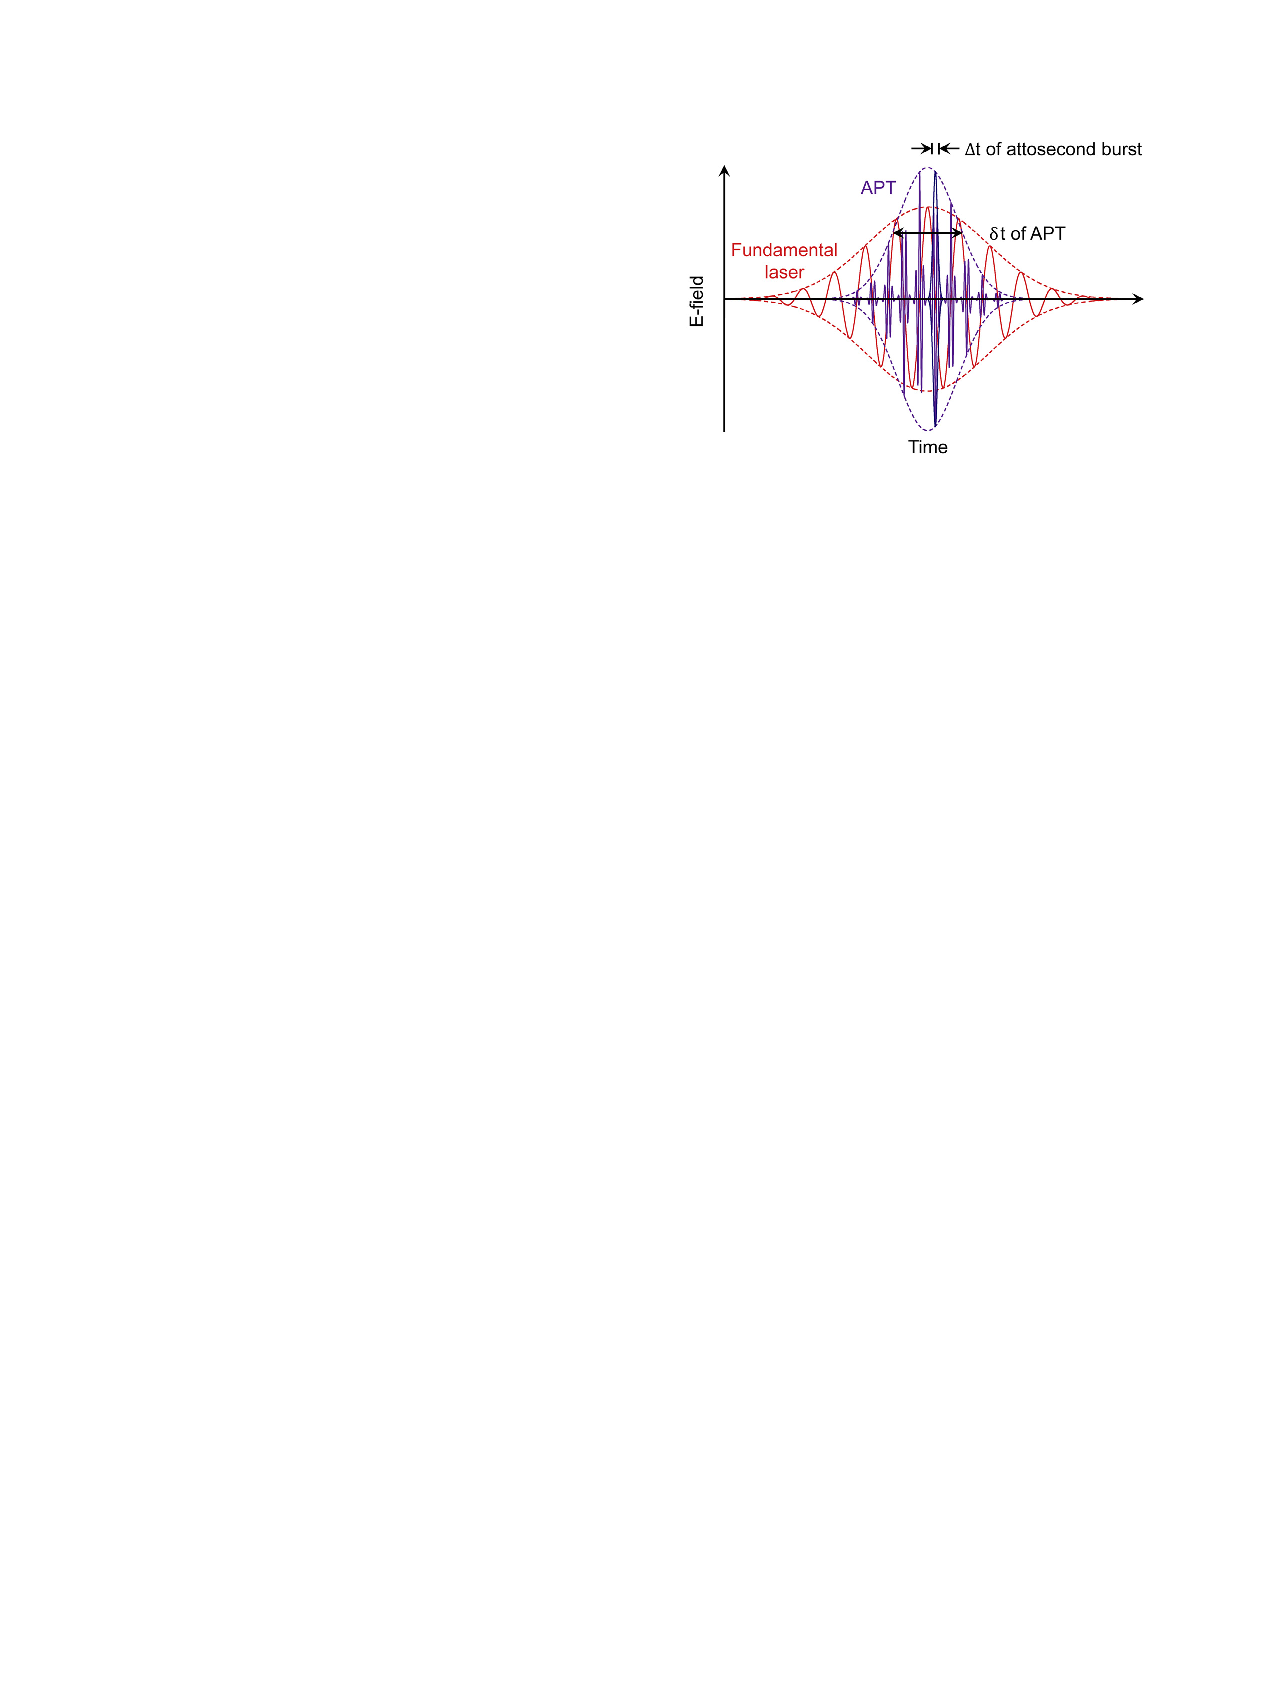
\includegraphics[width=0.4\textwidth]{figures/chap1/eich_APT_a.pdf}
		\label{fig:APT_time_domain}}
	\qquad
	\subfloat[]{
		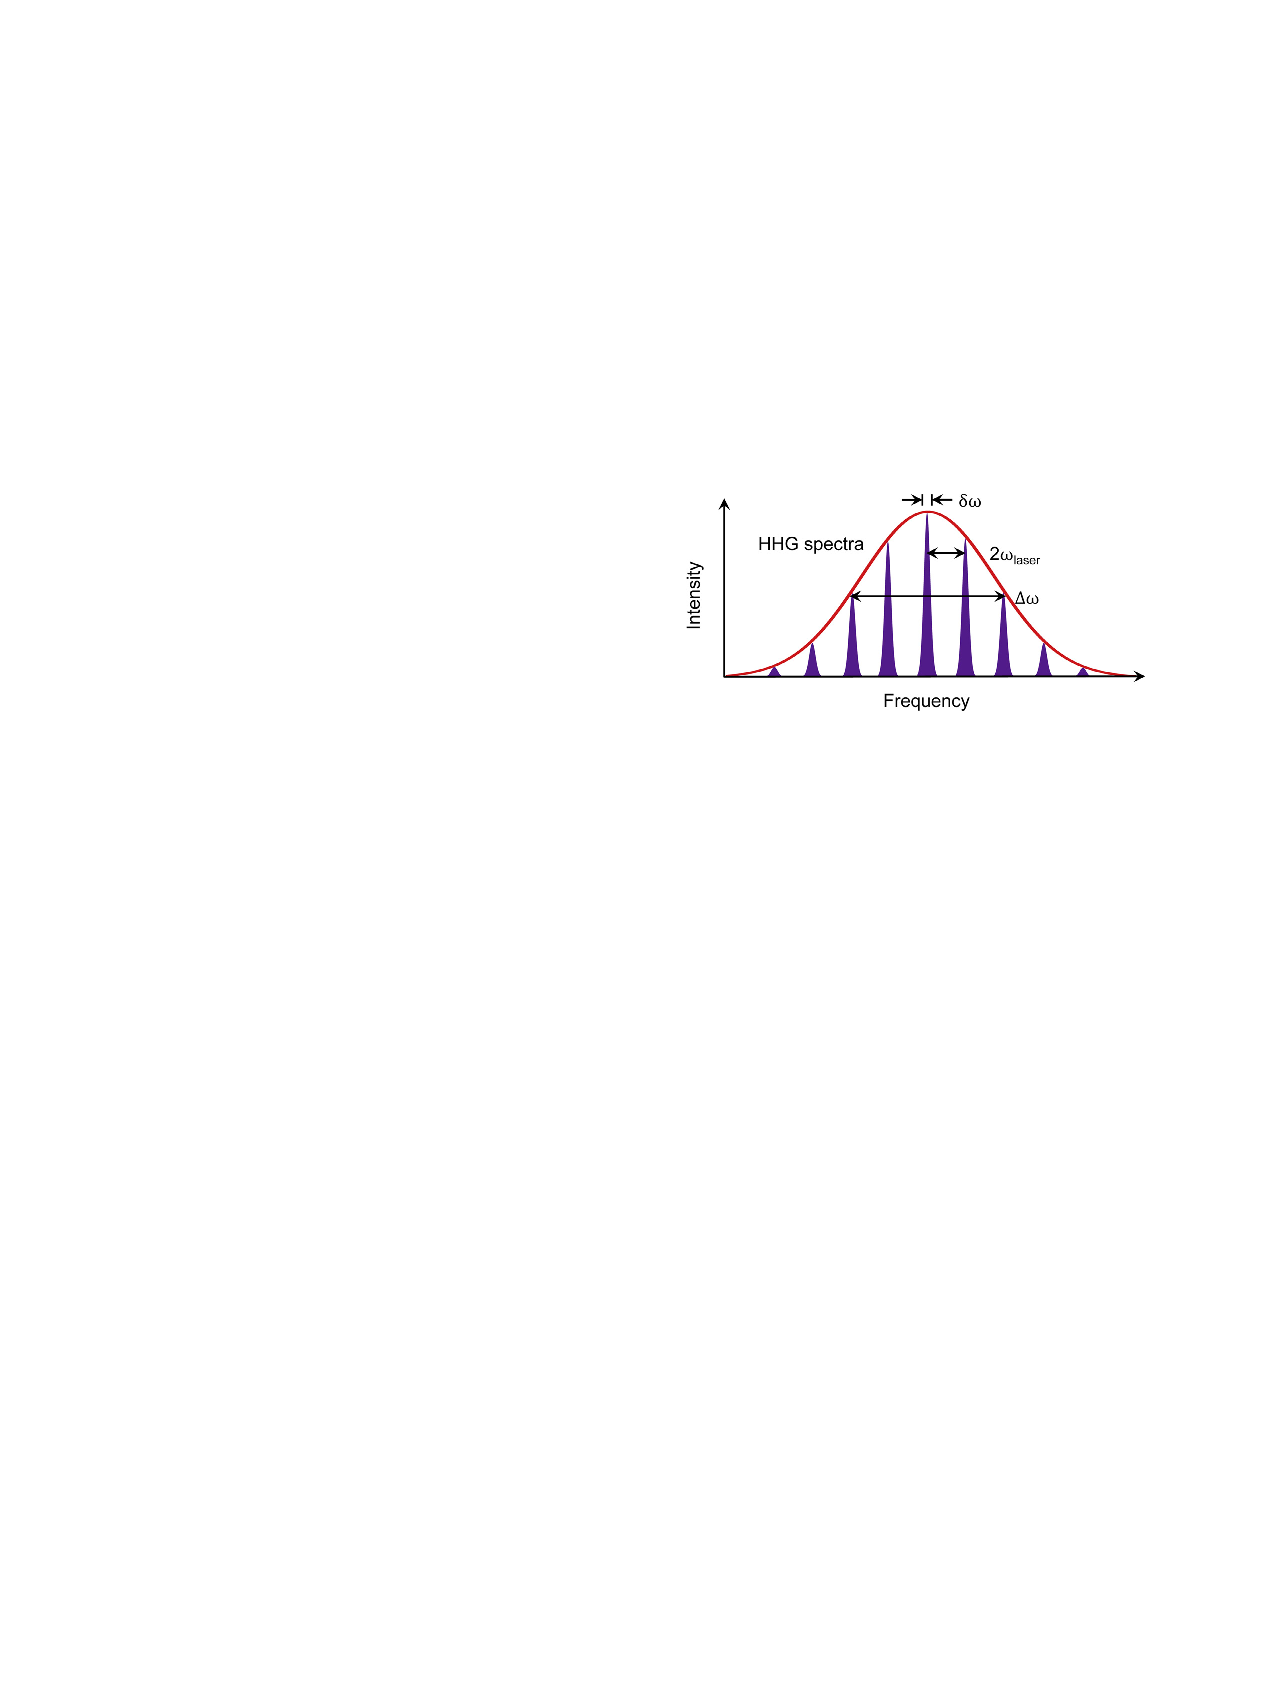
\includegraphics[width=0.4\textwidth]{figures/chap1/eich_APT_b.pdf}
		\label{fig:APT_freq_domain}}
	\caption{Time and frequency domain pictures of HHG. Figure adapted from \cite{eichTimeAngleresolvedPhotoemission2014}.}
	\label{fig:APT_IR_field}
\end{figure}

We start with a microscopic picture of harmonic generation, focusing on the interaction between a single atom and the laser field. In the early 1990s, a semi-classical model was developed to describe the process of high harmonic generation in three discrete steps: ionization, classical propagation in the vacuum, and recombination \cite{schaferThresholdIonizationHigh1993,corkumPlasmaPerspectiveStrong1993}. This model accurately predicts many of the fundamental features of HHG.

In the three step model, the electric field strength is on the order of the atomic potential that binds the electron to its parent atom. The valence electron's wavepacket evolves subject to the sum of the shielded Coloumb field and the spatially varying laser field. The electron can tunnel out of the distorted Coloumb field, as shown in the left panel of \cref{fig:ThreeStepModel}. This step is most likely to occur at the peak of the field, which occurs every half-cycle of the laser period.

The recently liberated electron is assumed to be born with zero initial kinetic energy. It accelerates in the oscillating laser field, gaining kinetic energy along the way, as shown in the central panel of \cref{fig:ThreeStepModel}. Its kinetic energy is proportional to the cycle-averaged quiver energy:
\begin{equation}
U_p = \frac{q_e^2 F_0^2}{4 m_e \omega^2} \propto I_0 \lambda^2
\label{eqn:Up}
\end{equation}
where $m_e$ is the electron mass, $q_e$ is the electron charge, $\omega$ is the frequency, $F_0$ is the electric field strength, $I_0$ is the intensity, and $\lambda$ is the wavelength of the laser. A more useful form of \cref{eqn:Up} is given below:
\begin{equation}
U_p \textrm{ [eV]} = \left( 9.33738 \times 10^{-5} \right) \times I_0 \textrm{[PW/cm\textsuperscript{2}]} \times \lambda\textrm{[nm]}^2
\end{equation}

The birth phase of the electron (relative to the laser period) determines its classical trajectory. Some electrons will be driven away from the parent ion, never to return; some will be driven back to the birth location, where they can scatter off of, miss, or recombine with the parent ion. We will only concern ourselves with those electrons that recombine (right panel of \cref{fig:ThreeStepModel}). Upon recombination, the electron will emit a photon of energy $I_p + KE$, where $I_p$ is the ionization potential of the atom and $KE$ is the kinetic energy acquired during the propagation step. A classical analysis of the electron propagation reveals that the maximum kinetic energy such an electron can gain is $3.17 U_p$, and therefore the maximum photon energy is: 
\begin{equation}
\hbar \omega_{cutoff} = I_p + 3.17 U_p
\label{eqn:cutoff_energy}
\end{equation}
This quantity is often called the cutoff energy, and it is proportional to $I_0 \lambda^2$. Thus, we can extend the maximum photon energy of the harmonics by increasing the fundamental wavelength of the laser.

Unfortunately, the brightness of an individual harmonic order will decrease strongly with increasing wavelength, with the intensity scaling between $\lambda^{-5}$ and $\lambda^{-6}$ \cite{tateScalingWavePacketDynamics2007,shinerWavelengthScalingHigh2009}. We can conceptually understand this as the compounding of two separate problems \cite{lewensteinTheoryHighharmonicGeneration1994}. First, longer wavelengths extend the cutoff energy, spreading a fixed harmonic conversion efficiency across more harmonics and lowering the brightness of each individual harmonic. This accounts for a factor of $\lambda^{-2}$. Secondly, the recombination probability scales inversely with square of the electron wavepacket spread that occurs during the propagation step. Longer wavelengths mean longer excursion times $\tau$, and the wavepacket spreads out as $\tau^{3/2}$. Since we are concerned with the harmonic intensity, we square this value to get $\tau^3 \propto \lambda^{-3}$. With this simple argument, we can see why the harmonic brightness should decrease as $\lambda^{-5}$.

So far, it appears that XUV spectrum is continuous in energy, ranging from $I_p$ to $\hbar \omega_{cutoff}$. This is because we have been considering the effects of a single-cycle laser pulse. In a multi-cycle pulse, the ionization-propagation-recombination steps will happen twice per pulse (every $T_0/2$ seconds), and each event results in a brief burst of light, as shown in \cref{fig:APT_time_domain}. If we Fourier transform this comb of attosecond pulses, we will get a comb in the frequency domain with separation $2 \omega_0$, as shown in \cref{fig:APT_freq_domain}. Thus, we expect to see only odd harmonics of the laser frequency $\omega_0$.

\subsection{Macroscopic Picture}

We now zoom out to the macroscopic picture, which encompasses the entire gas-laser interaction volume. In the far field, the radiation from individual atoms will be coherently summed to form an bright XUV light source. The overall efficiency of the HHG process depends on the phase mismatch $\Delta k$ of the individual dipoles across the interaction volume. We will see how the phase matching determines optimal interaction pressures for a given driving wavelength. Additionally, we will see the effect of XUV reabsorption by the gas on the overall XUV brightness.

\subsubsection{Phase Matching}

HHG will be an efficient process if the wave vector mismatch $\Delta k$ of the independent dipoles is zero. The phase mismatch term can be expressed as three separate factors, each arising from distinct physical phenomena \cite{rothhardtAbsorptionlimitedPhasematchedHigh2014}:
\begin{equation}
\Delta k = \Delta k_{disp} + \Delta k_{Gouy} + \Delta k_{dipole}
\label{eqn:phase_mismatch}
\end{equation}
The first term represents the dispersion from the generating medium. It has contributions from both the neutral atoms and the free electrons:
\begin{equation}
\Delta k_{disp} = \frac{2 \pi q}{\lambda} \frac{p}{p_0} \Delta \delta \left( 1 - \frac{\eta}{\eta_c} \right)
\end{equation}
Here, $q$ is the harmonic order, $\Delta \delta$ is the difference of the refractive indices of the fundamental and high order harmonic, $p_0$ is the standard pressure (1013 mbar), $p$ is the interaction pressure, $\eta$ is the ionization fraction and $\eta_c$ is the critical ionization fraction (the fraction at which the plasma dispersion of the free electrons exceeds the atomic dispersion).

The second term is the geometrical phase mismatch caused by focusing:
\begin{equation}
\Delta k_{Gouy} = q \pdv{\varphi_{Gouy}}{z} = q \pdv{z} \left( - \arctan \left( \frac{z}{z_R} \right) \right)
\label{eqn:deltak_Gouy}
\end{equation}
Here, $z_R = \pi w_0^2 / \lambda$ is the Rayleigh range and $z=0$ corresponds to the focal plane. Note that $\Delta k_{Gouy}$ is negative for all values of $z$. The atomic term arises from the intensity-dependent dipole phase acquired during the electron excursion \cite{lewensteinTheoryHighharmonicGeneration1994,balcouGeneralizedPhasematchingConditions1997,salieresCoherenceControlHighOrder1995}:
\begin{equation}
\Delta k_{dipole} = - \alpha_q \pdv{I}{z}
\label{eqn:deltak_atomic}
\end{equation}
The value of $\alpha_q$ depends on the quantum trajectory the electron takes during its excursion. For short trajectories, {$\alpha_q = 2 \times 10^{-14}$ cm\textsuperscript{2}/W} and for long trajectories, {$\alpha_q = 22 \times 10^{-14}$ cm\textsuperscript{2}/W} \cite{kazamiasPressureinducedPhaseMatching2011,balcouQuantumpathAnalysisPhase1999}. The sign of $\Delta k_{dipole}$ is positive (negative) if the gas source is located upstream (downstream) of the focus.

Experimentally, the phase matching can be adjusted by tuning the laser parameters (wavelength $\lambda$, intensity $I$, pulse duration, focal spot size $w_0$), the gas species ($I_p, n$ and $k$) and interaction pressure $P$, and the gas location relative to the laser focus ($z$). Additionally, a variable aperture (iris) located just before the generation lens effectively tunes multiple laser parameters simultaneously, and is known colloquially as ``the magic iris trick" \cite{kazamiasHighOrderHarmonic2002}. Because $\Delta k$ is dependent on the harmonic order $q$, it is impossible to perfectly phase match the entire harmonic spectrum simultaneously. As a result, we adjust the phase matching parameters to optimize the useful part of the harmonic spectrum, usually at the expense of the rest of the spectrum.

Also note that the dispersion phase can be controlled by tuning the interaction pressure $p$, while the other terms are (to first order) pressure independent. If the gas medium is at focus, $\pdv{I}{z} = 0$ and therefore $k_{dipole}=0$. In this case, the condition $\Delta k = 0$ can be met by setting to the pressure to an optimal phase matching pressure $p_{opt}$ \cite{rothhardtAbsorptionlimitedPhasematchedHigh2014}:
\begin{equation}
p_{opt} = p_0 \frac{\lambda^2}{2 \pi^2 w_0^2 \Delta \delta \left( 1 - \frac{\eta}{\eta_c} \right)}
\label{eqn:phase_matching_pressure}
\end{equation}

We therefore arrive at the conclusion that the optimal phase matching pressure scales with the square of the fundamental wavelength. Furthermore, tighter focusing ($w_0 \rightarrow 0$) and higher ionization fractions ($\eta \rightarrow \eta_c$) require larger pressures. Therefore, creating bright harmonics from a long wavelength, relatively weak pulse requires significantly higher interaction pressures than a strong 800 nm pulse. This is the motivation for designing a vacuum system and gas source that can deliver high interaction pressures.

\subsubsection{XUV Reabsorption}
\label{sec:XUV_reabsorption}

\begin{figure}
	\centering
	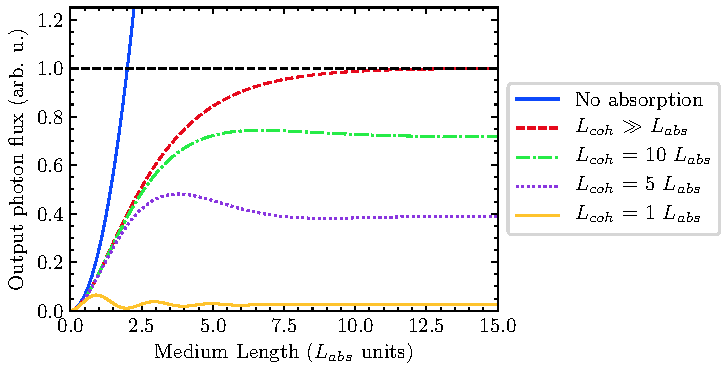
\includegraphics[width=0.75\textwidth]{figures/chap1/Constant1999_fig1.pdf}
	\caption{1D absorption model from \cref{eqn:HHG_Nout_simple}.}
	\label{fig:Constant1999_fig1}
	% created with \Python Scripts\HHG_Phasematching-master\test\Constant_fig1.py
\end{figure}

We now consider the effects of XUV absorption on the phase matching process using the 1-dimension model introduced by Constant et. al. \cite{constantOptimizingHighHarmonic1999}. In doing so, we restrict ourselves to the on-axis emission of the $q$\textsuperscript{th} harmonic. That is, we consider only harmonics with a wave vector $k_q$ that is collinear to the fundamental ($k_0$). In this case, the number of photons emitted per unit time and area is:
\begin{equation}
N_{out} = \frac{\omega_q}{4 c \epsilon_0 \hbar} \left| \left[ \int_{0}^{L_{med}} \dd{z} \rho(z) A_q(z) \exp \left( - \frac{L_{med} - z}{2 L_{abs}}  \right) \exp \left( i \varphi_q(z) \right)  \right] \right|^2
\label{eqn:HHG_Nout}
\end{equation}
Here, $\rho(z)$ is the gas medium density, $A_q(z)$ is the amplitude of the harmonic response at frequency $\omega_q$ and $\varphi_q$ is its phase at the exit of the medium, which has length $L_{med}$. If we are using a loose focusing geometry, then the gas density and harmonic response amplitude are constant along the interaction volume: $\rho(z) = \rho$ and $A_q(z)=A_q$. With this restriction, \cref{eqn:HHG_Nout} evaluates to:
\begin{equation}
\begin{aligned}
N_{out} = & \\ \rho^2 A_q^2 & \frac{4L_{abs}^2}{1+4\pi^2(L_{abs}^2 / L_{coh}^2)} \left[ 1 + \exp\left(-\frac{L_{med}}{L_{abs}}\right) - 2 \exp\left(\frac{\pi L_{med}}{L_{coh}}\right) \exp\left(-\frac{L_{med}}{2L_{abs}}\right) \right]
\label{eqn:HHG_Nout_simple}
\end{aligned}
\end{equation}
Here, we use the notation $L_{coh} = \pi/\Delta k$ for the coherence length ($\Delta k = k_q - q k_0$) and $L_{abs} = 1/{\sigma \rho}$ for the absorption length.


\cref{eqn:HHG_Nout_simple} is plotted in \cref{fig:Constant1999_fig1}. In the case of no absorption ($L_{abs} \rightarrow \infty$), the harmonic yield grows as $L_{med}^2$. Otherwise, the optimized conditions are $L_{med} > 3 L_{abs}$ and $L_{coh} > 5 L_{abs}$.

Experimentally, $L_{med}$ is fixed by the geometry of the gas source, $L_{abs}$ is directly controlled by adjusting the backing pressure, and $L_{coh}$ is indirectly controlled by other parameters (gas source position relative to focus, focusing conditions, iris diameter, etc.). In \cref{sec:HHG_gas_sources}, we will apply this simple model to the gas sources available in our lab to maximize our HHG yield.

\textbf{to do:}

now, find out where you are on this plot for the different gas cell geometries. that is, free jet, LPC and HPC have set medium lengths. given their pressure performance, you can calculate the range of interaction pressures achievable by each HHG source, and therefore you can calculate the Labs for a specific generating gas (Ar, for example). having done that, you know the Labs and the Lmed, so you know the x-axis position. you still don't know the coherence length, but it's a start.

motivation: in the LPC, we can't see pressure rollover. this plot helps show why. (assuming the LPC and the free jet are still on the rising edge of the curves). this plot explains why.

\begin{appendices}
\chapter{Guidelines for using the TABLe}
\label{appendix:TABLe_manual}

\section{OMRON Pump-down Procedure}

Special thanks for Andrew Piper for coding and installing the \OMRON safety system. Below is an operational guideline to pump the system down to UHV using the \OMRON system. Please see Andrew Piper's \OMRON manual for additional details on the microcontroller system.

This procedure assumes that the chambers are initially at atmospheric pressure, the rough pumps are turned on, and the solenoid shutoff valves on the roughing line are closed.

\begin{enumerate}
	\item Seal and isolate all chambers. Close the manual hand valves between each turbo pump and the solenoid shutoff valves. Reattach any blow-off flanges (KF-25 blanks) that may have come off from the previous venting cycle.
	\item Ensure the \OMRON's \, safety system is engaged by attempting to open one of the pneumatic gate valves via the control panel. \textbf{Caution: operating a gate valve between two chambers with a pressure differential can cause catastrophic system failure! Only perform this step after you have verified that all chambers are at atmospheric pressure!} If the gate valve opens while both chambers are above the upper setpoint, then the \OMRON \, safety system has been disabled. Enable the safety system by switching the override switch to OFF.
	\item Retract the metal filters from the beam path to protect them from potential pressure surges. 
	\item Initiate the pump-down sequence by pressing the OK button on the \OMRON. This will open all solenoid valves simultaneously with a loud \textit{thunk!}
	\item Slowly open the manual handvalves while monitoring the pressure load on the rough pumps to avoid overloading the rough pump system. Use the two Raspberry Pi remote pressure monitoring systems to monitor the inlet pressure for each blower system. As a rule of thumb, try to keep the inlet pressure below $\approx$100 Torr during this step. \textbf{Warning: overloading the rough pumps will result in pump oil being expelled into the rough pump's exhaust line. Continuing to run in this condition can lead to overheating and eventually seizing of the rough pump.}
	\item Once the hand valves are fully open on all chambers, you can turn each blower system ON to accelerate the remaining pump-down procedure.
	\item Power on the turbo power supplies and switch the turbos to ON. After a few seconds, the magnetically levitated turbos will start levitating with a soft \textit{thunk!}.
	\item Each turbo will automatically start spinning when its chamber reaches the upper set point (about 200 mTorr). The turbos will take a few minutes to reach their final speed.
	\item Wait for the system to pump down. It typically takes 15-45 minutes for the entire system to reach $10^{-6}$ Torr.
	\item The pneumatic gate valves for adjacent chambers will be enabled when both chambers are below their lower setpoint pressure (about $5 \times 10^{-6}$ Torr). Once all chambers are below their lower setpoints, the \OMRON considers the system is to be fully pumped down.
	\item ARM each chamber by pressing ESC + [chamber number]. The \OMRON's display will update to show which chambers are armed (G: generation \& differential pump chambers, M: mirror chamber, T: target chamber, S: photon spectrometer chamber).
\end{enumerate}

\section{OMRON Venting Procedure}

The \OMRON \ system was designed with the ability to vent any single chamber or combination of chambers while keeping the others pumped down. This was a possibility when each chamber had its own rough pump, but now that the mirror, target \& spectrometer chambers share a single blower system, extra care must be taken. \textbf{Any chambers that share a backing rough pump must be vented simultaneously to avoid turbopump overload.} For example, the mirror chamber, target chamber and spectrometer share a common blower system, and attempting to vent the one chamber while keeping the others will result in the spectrometer's turbo pump crashing due to the high backing pressure in the rough line.

This procedure assumes an initial condition of all chambers pumped down to UHV with the turbos running.

\begin{enumerate}
	\item Turn off all gas sources / loads. If the HPC is installed, follow the HPC shutdown procedure.
	\item Turn off the blowers.
	\item Block the laser into the interferometer.
	\item Close the pneumatic gate valves.
	\item Disarm the chambers by pressing ESC + [chamber number].
	\item Verify the \OMRON's safety system is not disabled by checking the bypass switch.
	\item Enable the venting valves by switching ON the vent \& purge controls on the control panel. The chambers will not vent without this step!
	\item Remove the KF clamps on the blow-off valves.
	\item Start the \OMRON \ venting script by pressing ALT + [chamber number] on the \OMRON.
	\item The user can now walk away from the system. It will take a few hours to vent.
\end{enumerate}

The venting script will immediately stop the turbopump's motors, open the solenoid venting valves after 30 seconds, close the roughing line's solenoid valves after 30 minutes, and close the solenoid venting valves after about 5 hours. The preceding timeline was chosen following the manufacturer's recommendation, and to avoid closing the roughing line's valves before the turbos had completely stopped spinning. 

\section{Aligning the Interferometer}
\label{app:aligning-interferometer}

\subsection{the generation arm}

\subsubsection{The Ellipsoidal Mirror}

\subsection{the pump arm}

\subsection{finding spatial overlap}

\subsection{finding temporal overlap}

\section{Pointing into the Interferometer}
\label{app:pointing-into-TABLE}

the importance of pointing into the interferometer - spatial and temporal alignment

\section{The High Pressure Cell (HPC)}

\begin{figure}
	\centering
	\includegraphics[width=0.9\textwidth]{figures/app1/HPC_outside_view.png}
	\caption{Exterior view of the generation chamber with the HPC installed showing the ancillary vacuum hardware. Red arrow indicates input laser path; green arrow points towards the HPC's RV pump.}
	\label{fig:HPC_outside_view}
\end{figure}

\begin{figure}
	\centering
	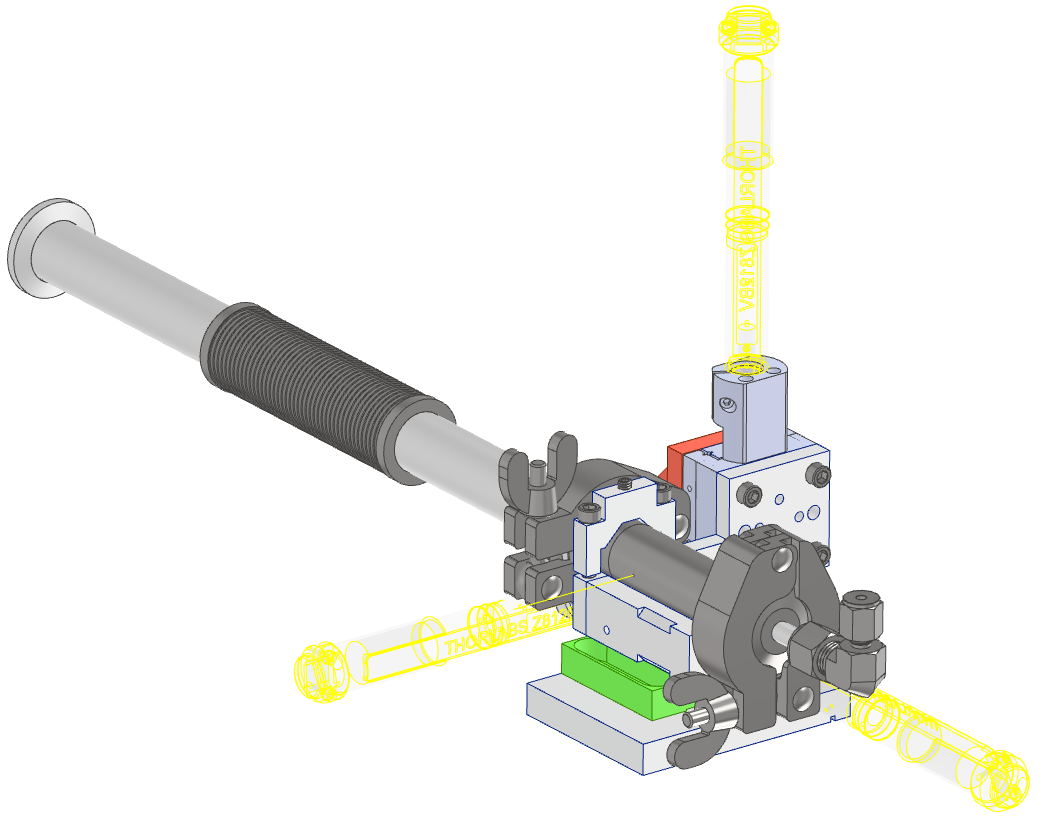
\includegraphics[width=0.9\textwidth]{figures/app1/HPC_on_stage2.png}
	\caption{The HPC with bracket installed on the XYZ translation stage, configured for the generation chamber. The hose clamp and gas supply tube is omitted from this drawing for clarity.}
	\label{fig:HPC_on_stage}
\end{figure}

\begin{figure}
	\centering
	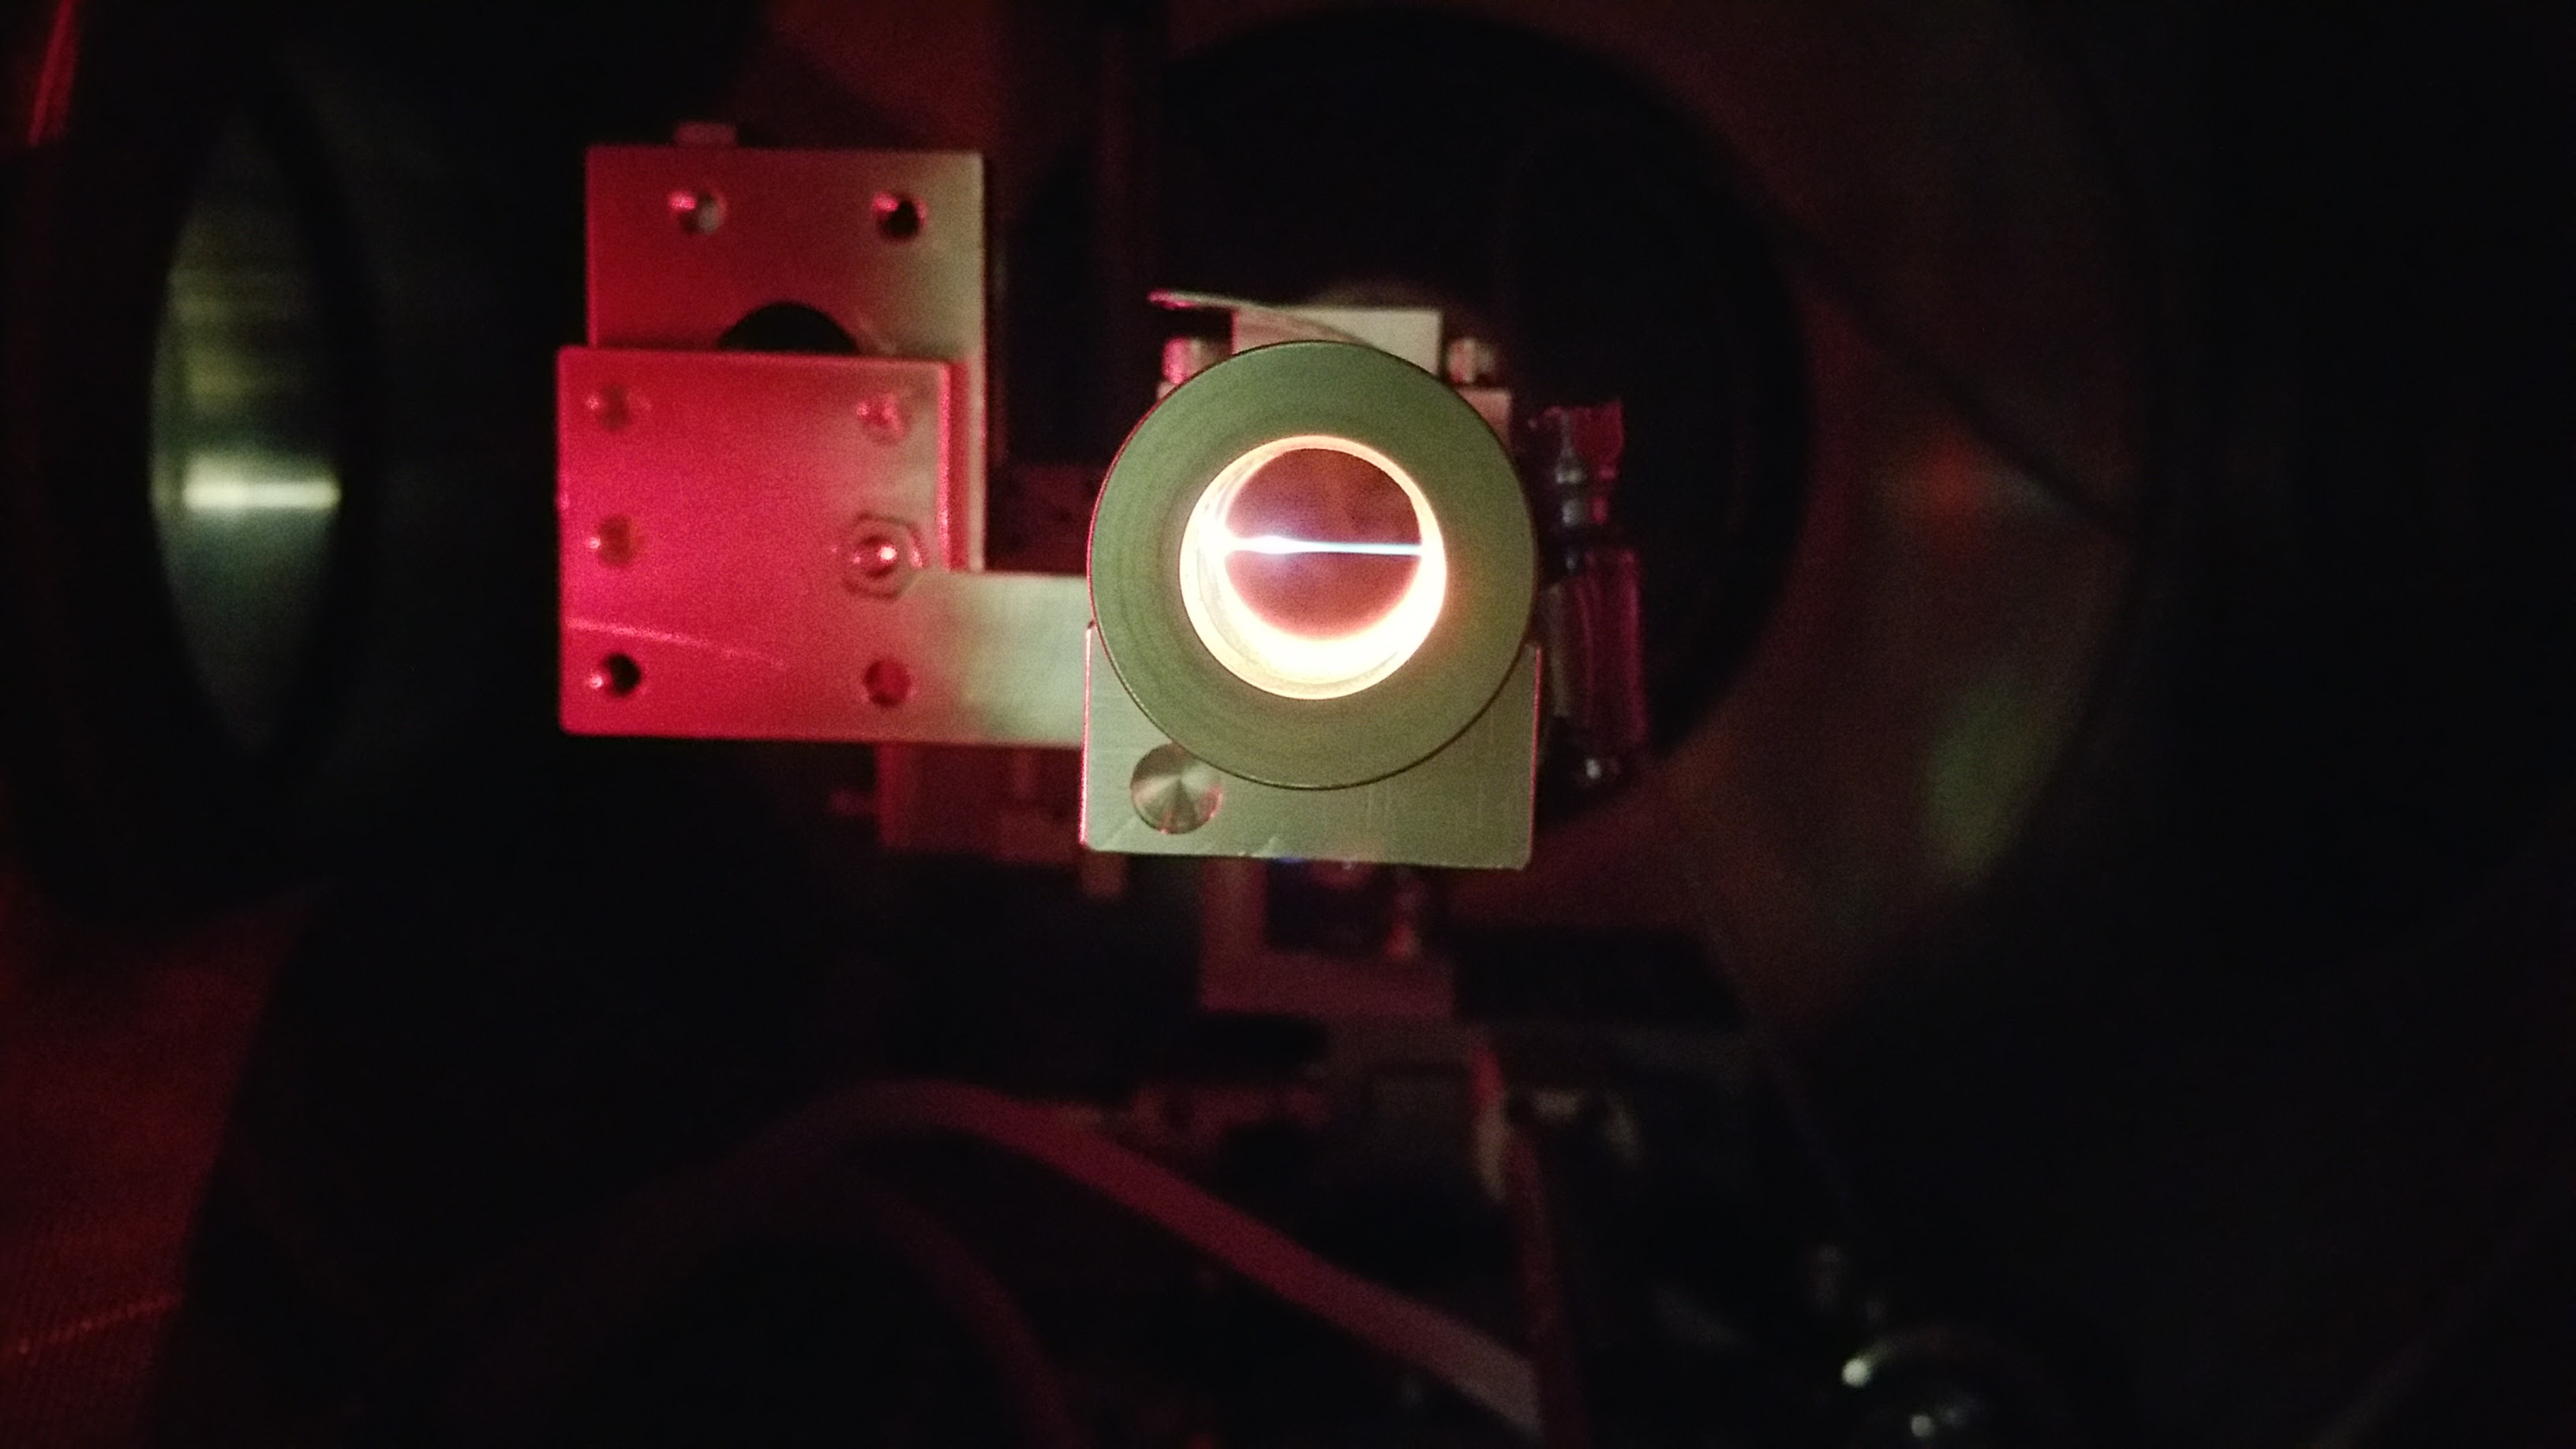
\includegraphics[width=0.75\textwidth]{figures/app1/HPC_outer_can_laser.jpg}
	\caption{Laser filament in the aligned outer pipe of the HPC. The inner pipe is not yet installed. Alignment of the outer pipe is done at very low intensities; after alignment the power was increased to create a filament for illustrative purposes only. This picture was taken in the target chamber during the initial testing of the HPC. The geometry of this chamber requires that the orientation of the mounting bracket is reversed compared to what is shown in Fig \ref{fig:HPC_on_stage}.}
	\label{fig:HPC_outer_can_laser}
\end{figure}

\begin{figure}
	\centering
	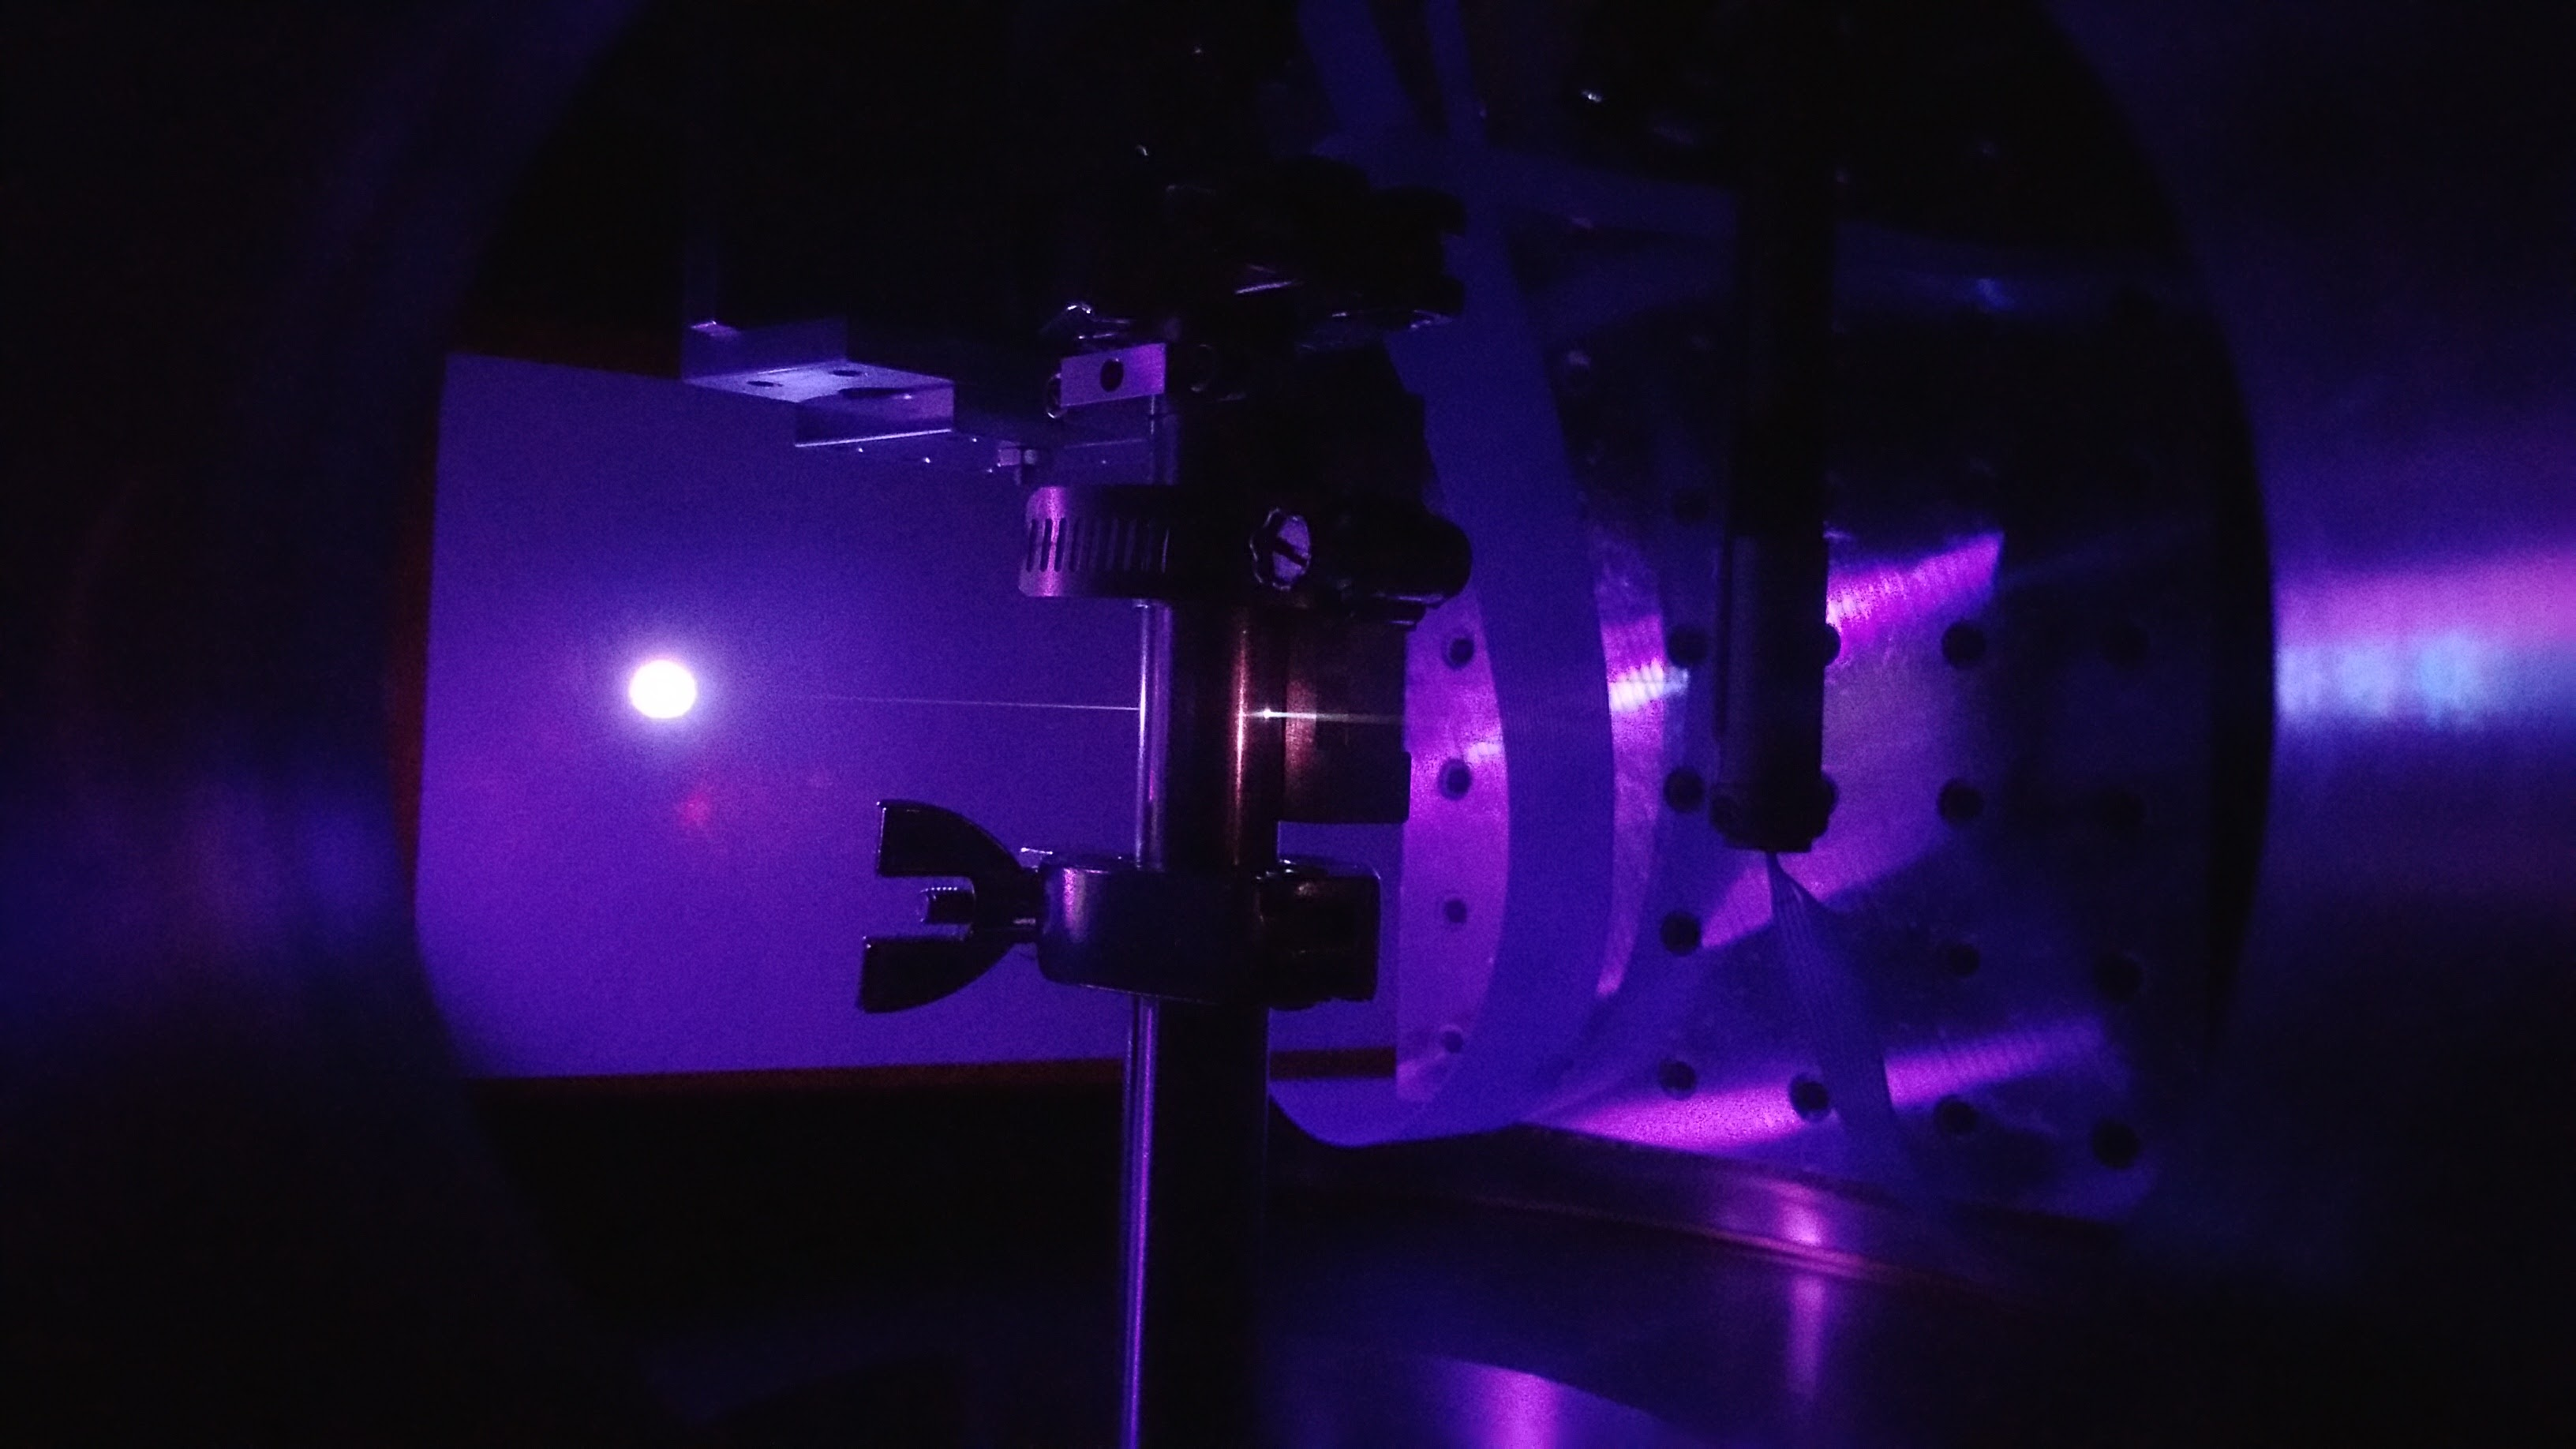
\includegraphics[angle=270, width=0.5\textwidth]{figures/app1/HPC_drilling.jpg}
	\caption{Laser drilling the inner pipe. A card blocks the laser after exiting the HPC. The HPC was pressurized with Ar gas to enhance the filament for illustrative purposes.}
	\label{fig:HPC_drilling}
\end{figure}

\subsection{Introduction}
\textit{main text: description of the HPC's design, pressure \& harmonic performance, pressure modeling, phase matching considerations. this section: how to install and actually use the HPC, how to machine or reorder certain parts.}

- focal length considerations. range of acceptable focal lengths. advantages of reflective vs transmissive focusing. possible schemes for shorter focal lengths. 

- space constraints of TABLe generation chamber limit the size of the XYZ stack. these are Newport 9066 1/2" travel stages, with 1" travel thorlabs motors (that's what we had, ideally you would use 1/2" motors). as a result, you can accidentally drive the motor more than the stage will allow. this will result in the motor falling out of the stage. in this case, you will have to immediately block the laser, vent the chamber, and reattach the motor. note: travel of all motors is from 0 to 14 mm.

- in-vacuum manipulation via the vacuum bellows (limits of motion, max pressure differential)

The ancillary vacuum hardware can be seen in Fig \ref{fig:HPC_outside_view}. A small oil-lubricated RV pump (not shown in this picture) provides differential pumping to the interior of the HPC. An inline Baratron diaphragm pressure sensor (effective range: 1 - 760 Torr) tracks the interior pressure of the edge-welded bellows. A manual gate valve is used to isolate the HPC from the RV pump when the additional pumping is not needed. Right angle KF fittings were used to route the HPC's vacuum line above the pump arm of the interferometer.


\subsection{Initial Installation and Alignment}
\label{app:initial-alignment-HPC}
First, a note about laser safety. The following alignment procedure should be done at the lowest possible laser power to minimize both accidental drilling of the HPC and the danger posed by stray light. Stray reflections or scatter from the many metallic surfaces of the HPC assembly pose a potential safety risk during alignment. The surface most likely to cause laser scatter is the front face of the outer pipe, which is roughened stainless steel located about 3/8" before the focus. The material's roughness and the negative radius of curvature of the incoming light make it unlikely that incident light will coherently focus to a point upon reflection. However, it is possible that the sidewall of the outer pipes's aperture could act as a focusing mirror. Additionally, the hose clamp or mounting bracket could coherently reflect light towards the user. The user is advised to strictly follow all laser safety protocols during this alignment procedure. Whenever possible, direct observation of the laser beam on the surfaces of the HPC should be avoided, instead a webcam should be used to view the interior of the generation chamber.

The initial installation of the HPC can be time consuming and tedious, but once installed it will retain its alignment for a period of weeks or months. The pointing into the cell should be done on a daily basis, but this is only slightly more complicated than what must be done with a free expansion gas jet.

Optically, the HPC cell consists of four pinhole apertures (diametrically opposed pinholes on both the inner and outer pipes) with the laser focus near the center of the inner pipe. The optical transmission of the HPC is therefore very sensitive to the relative alignment of these components, as well as the pointing of the laser into the HPC. To simplify the alignment, the two innermost holes are laser drilled \textit{in-situ} after the outer pipe has been aligned. To maintain the relative alignment of the inner \& outer apertures, the user should refrain from adjusting the inner pipe after the initial alignment is completed. Therefore, daily alignment of the HPC should be performed using only the in-vacuum motorized XYZ stages.

The first step of the HPC installation is installing the rough vacuum feedthrough flange. The TABLe's generation chamber uses a custom flange (a 4.5" CF blank with a KF16 half nipple welded to the air-side and a KF16 bulkhead groove \& tapped holes machined into the vacuum side). To accommodate the length of the in-vacuum bellows, we use a custom 10" CF to 4.5" CF reducing nipple (OAL = 4.25"), which acts as a spacer between the feedthrough flange and the KF16 flange on the HPC. Although it was absent from the original design, a spacer 4.5" CF flange (thickness = 0.68") between the feedthrough and the reducing full nipple is used to relax the compression in the bellows and allow for a larger range of motion. For convenience, the user should install the edge-welded bellows to the bulkhead flange before installing the flange on the chamber.

The supporting bracket for the HPC was designed to be interchangeable with the free gas nozzle's bracket. This design, shown in Fig. \ref{fig:HPC_on_stage}, allows the user to change the gas source type without disturbing the alignment of the XYZ stage to the optical axis. For completeness, we will assume that the XYZ stage has been misaligned or removed from the chamber. First, the user should align the laser to the interferometer so that the laser path in the generation chamber can be used as a reference. Then, the stage should be positioned in the chamber so that the focus is roughly in the center of the stage's motion. Finally, the stage's z-direction should made parallel to the optic axis. This can be done by tracking the position of the laser on a card mounted to the stage while moving the stage upstream and downstream of the focus. After clamping the stage to the breadboard, check that the alignment is still true before continuing to the next step.

The next step is to align the outer pipe of the high pressure cell by maximizing its light transmission. This is best done in two steps: first, coarse alignment is done visually at low power (insufficiently intense to laser drill the pipe), followed by fine adjustments using a power meter at moderate intensities (above the noise floor of the power meter). Note that accidentally drilling out the outer pipe will reduce its differential pumping performance. Given the chamber's small size, it is not practical to place a power meter in the generation chamber after the focus during the alignment procedure. Rather, it is preferable to divert the beam out of the vacuum system using the linear actuator \& silver mirror assembly located approximately 85 cm downstream of the focus.\footnote{Special thanks to Eric Moore for designing and installing this optomechanical component.} When inserted, the linear actuator intersects the beam path and redirects the beam out of the vacuum system through a window onto the upper deck of the optical table. The beam size can be reduced using a focusing lens onto the face of a power meter. Note that for most generation focusing conditions, the large beam size at the diverting mirror makes this beam path lossy. To accurately calculate the transmission through the HPC, it is necessary to measure the power immediately after the HPC in the generation chamber.

For the coarse alignment, the input beam intensity should be reduced using an upstream iris, to the point that it is barely visible near the focus. Since a tightened KF connection prevents rotation of the components, the alignment of the outer piper is done prior to making any KF connections. However, the KF clamps should be fitted on either end of the pipe to ensure that there is enough room to make the connections without disturbing the alignment once finished. The outer pipe should be placed in its cradle, with the aluminum \& hose clamps made snug around the pipe but not taut.\footnote{The HPC's XYZ assembly and bracket were designed for the TABLe generation chamber. If it is being installed elsewhere, the user should verify that the height is correct. When installed correctly, the bottom of the Z-motor range should correspond to the HPC lowered completely out of the way of the laser; the top of the range should correspond to the laser going through the center of the HPC, with about 1 mm to spare.} Transmission should be optimized by iteratively tuning the following parameters: (1) rotation of the pipe in the cradle, (2) height of the cradle using the vertical motor, and (3) horizontal (transverse) position of the assembly using both the horizontal motor and the position of the pipe in the cradle. For fine adjustment, the iris should be adjusted so that the power meter reads about 20-30 mW when measured after the linear actuator.\footnote{This power is appropriate for a 1kHz repetition rate and a generation focal length of 30 or 40 cm.} The clamps should be tightened so that movement of the pipe is possible, but difficult. The area around the power meter should be covered to prevent air currents from affecting the measurement. The transmitted power should be optimized using the same procedure as before.

Once the outer pipe is aligned, tighten all connections and connect the bellows to the outer pipe. Check that the alignment has not been changed by torquing these connections. Verify that the unattenuated laser beam can pass through the outer pipe without interference, as shown in Fig. \ref{fig:HPC_outer_can_laser}. If everything looks good, we can proceed to install the inner pipe.

First, attach the gas delivery feedthrough flange onto the HPC assembly without the inner pipe. Being mindful to not disturb the alignment of the outer pipe, check that the gas delivery tubing does not interfere with the laser path. Remove the gas delivery feedthrough flange, cut the inner pipe to length (OAL = 1.75"), and make the Swagelok connection between the inner pipe and the KF feedthrough. Make sure the inner pipe is normal to the flange's sealing surface, otherwise the laser will skim the sidewall of the inner pipe rather than go through the center. Install the gas delivery assembly onto the HPC assembly by tightening the KF clamp.

Laser drilling the inner pipe will sputter a significant amount of metal onto the inner surfaces of the chamber. Since the active drilling surface is on the upstream face of the pipe, most of the material will go upstream. Therefore, the laser window needs to be swapped out for a "sacrificial" window prior to drilling.\footnote{After drilling, the sacrificial window will be completely coated with a thin metal film. Most of the metal can be removed using methanol, but don't expect to be able to use the window for anything but laser drilling. Using a window with different optical properties (i.e., thickness or material), or no window at all, will change the pointing and effective focal length of the beam. It has been suggested that the laser window could be protected by placing a thin sheet of transparent plastic (Saran Wrap) between the window and the HPC, but we haven't tested this method.} Out of an abundance of caution, close the gate valve to the mirror chamber, retract the linear actuator \& silver mirror from the beam path, and block the generation chamber's vacuum aperture with a card.

Laser drilling should be done with the appropriate safety precautions: wearing laser goggles, notifying fellow labmates of your activity, and posting signs on the entrances to the lab. The user can cover up the chamber's flanges and set up a webcam to remotely monitor the laser drilling status to minimize the risk of inadvertent laser exposure.

At this point, the actual process of laser drilling is quite simple. There is no way to control the exact positioning of the inner pipe relative to the outer pipe, so there are no adjustments to make. Rather, the design relies on the mechanical alignment of the inner pipe relative to the outer pipe, which is ultimately set by the gas feedthrough weld, the Swagelok and the KF fitting. On the other hand, a used inner pipe cannot be reinstalled to the HPC once it is removed, since alignment is effectively impossible. To laser drill the pipe, simply let the unattenuated beam into the chamber and wait a few minutes until the laser emerges from the exit of the HPC. See Fig. \ref{fig:HPC_drilling}.

If you are planning on scanning the k-direction of the HPC during an experiment, you should do so now while you are set up for laser drilling. Similarly, if you are using a non-reflective (achromatic) focusing scheme and are planning on changing wavelengths during your experiment (which will change the effective focal length), you should step through the full range of wavelengths while drilling. Doing so will open up the apertures slightly, resulting in additional metal deposition on the sacrificial laser window.

After laser drilling is complete, reinstall the laser window and verify the HPC has retained its alignment.



\subsection{Alignment with the HPC Installed}

The daily pointing procedure, described in \ref{app:pointing-into-TABLE}, is largely unchanged by the presence of the HPC. However, there are some extra considerations that need to be made if the HPC is installed. The small apertures of the HPC and the non-linear nature of HHG demand high accuracy in the pointing into the cell, so small corrections to the positioning of the HPC have to be made after the daily pointing procedure is completed.

\subsubsection{Pointing into the Interferometer}
If the interferometer is already aligned, the presence of the HPC does not really complicate the daily procedure of the beamline. In this case, the user should block the laser into the generation chamber and align the pointing into the interferometer using the pump arm, as usual.\footnote{Failure to block the laser prior to changing the pointing may result in laser-drilling the HPC.} The procedure described in \ref{app:pointing-into-TABLE} is sufficiently accurate to get the laser through the HPC, but it won't necessarily yield optimized harmonics. Rather, the user may have to make small tweaks to the transverse position of the HPC. This can be done by optimizing the harmonic flux by making small (10 - 25 $\mu$m) steps using both the vertical and horizontal HPC motors while monitoring the harmonic yield using a fast camera exposure ($< 0.5$ s). In our experience, the optimal HPC position is typically within 50 $\mu$m of the previous day's position.

The HPC's apertures may no longer be circular if the HPC has been subjected to accidental laser drilling or significant laser drift. Non-circular apertures may result in a complex spatial profile of the harmonics, which can make the optimization of the harmonic yield difficult.

\subsubsection{Aligning the Interferometer}
If the interferometer needs to be realigned, then the HPC must be lowered out of the way of the laser. This is because the spatial mode of the IR is distorted by the HPC's apertures, which can introduce small shifts in the pointing of the IR after the HPC. Once the HPC is out of the way, the alignment procedure described in \ref{app:aligning-interferometer} can be followed without modification. Unless major changes were made to the interferometer, the angle of the HPC's apertures should remain aligned to the k-vector of the generation arm. In this case, the optimal position of the HPC can be found by maximizing the transmitted power of an the attenuated laser through the HPC, as described in the latter part of \ref{app:initial-alignment-HPC}. If major modifications were made to the interferometer, the user should consider aligning the HPC from scratch.


\subsection{Pump Down Procedure}



- pump down procedure

- generating and optimizing harmonics

- max internal pressure / pressure differential of the bellows tube

- max displacement of the tube

\subsection{Startup and Shutdown}


\section{Laser System Specifics}
importance of pointing \& laser performance for our experiments

\subsection{The Spitfire}
\subsubsection{Regular Maintenance}
- cleaning the stretcher

- increasing the pump laser currents

- changing the chiller fluid, desiccants, etc

\subsubsection{quirks and features}
- regen cavity tweaks

- photodiode problems

- software issues - bugs and troubleshooting

\subsection{Pointing Stabilization into the External Compressor}
- dietrich plots for pointing
\subsection{The Spitfire's External Compressor}
\subsubsection{external compressor alignment}
\subsubsection{cleaning the grating}

\subsection{The TOPAS-HE}
- aligning
- importance of power stability and pointing stability

\subsection{stability}
- boxing things up
- power stability throughout the day, people in the lab
- unstable harmonic yield from the HPC at high pressures
\section{The Shutter System}

\section{The Vacuum System}
- blower upgrade

- remote pressure sensing

- vacuum calculations for steady state pressure of beamline

\section{Best practices: data acquisition}

read-out noise from camera. (how noise scales)

\section{Steve's sections}
steve - grating alignment (which axes do what to harmonics?)

steve - 2-source / phase plate stuff, including calibration

steve - operating the cage and crank 
\end{appendices}

\backmatter
% We use BIBTeX for the bibliography---you don't have to
% \nocite{*} % To display all refs, even uncited refs (useful when editting)
\bibliography{templatebib}
\bibliographystyle{unsrt} % use your favorite BIBTeX style

% If for some reason you are anti-BIBTeX, then you would use the
% following instead of the above:
%\begin{thebibliography}{99}
% ...
%\end{thebibliography}


% Note: GS 2010 requires bibliography/references _before_ the appendix
% if you believe their guidelines; however, conversations with GS
% staff suggests _they don't care_. Go figure. So do what you like.

%\appendix
%\chapter{Guidelines for using the TABLe}
\label{appendix:TABLe_manual}

\section{OMRON Pump-down Procedure}

Special thanks for Andrew Piper for coding and installing the \OMRON safety system. Below is an operational guideline to pump the system down to UHV using the \OMRON system. Please see Andrew Piper's \OMRON manual for additional details on the microcontroller system.

This procedure assumes that the chambers are initially at atmospheric pressure, the rough pumps are turned on, and the solenoid shutoff valves on the roughing line are closed.

\begin{enumerate}
	\item Seal and isolate all chambers. Close the manual hand valves between each turbo pump and the solenoid shutoff valves. Reattach any blow-off flanges (KF-25 blanks) that may have come off from the previous venting cycle.
	\item Ensure the \OMRON's \, safety system is engaged by attempting to open one of the pneumatic gate valves via the control panel. \textbf{Caution: operating a gate valve between two chambers with a pressure differential can cause catastrophic system failure! Only perform this step after you have verified that all chambers are at atmospheric pressure!} If the gate valve opens while both chambers are above the upper setpoint, then the \OMRON \, safety system has been disabled. Enable the safety system by switching the override switch to OFF.
	\item Retract the metal filters from the beam path to protect them from potential pressure surges. 
	\item Initiate the pump-down sequence by pressing the OK button on the \OMRON. This will open all solenoid valves simultaneously with a loud \textit{thunk!}
	\item Slowly open the manual handvalves while monitoring the pressure load on the rough pumps to avoid overloading the rough pump system. Use the two Raspberry Pi remote pressure monitoring systems to monitor the inlet pressure for each blower system. As a rule of thumb, try to keep the inlet pressure below $\approx$100 Torr during this step. \textbf{Warning: overloading the rough pumps will result in pump oil being expelled into the rough pump's exhaust line. Continuing to run in this condition can lead to overheating and eventually seizing of the rough pump.}
	\item Once the hand valves are fully open on all chambers, you can turn each blower system ON to accelerate the remaining pump-down procedure.
	\item Power on the turbo power supplies and switch the turbos to ON. After a few seconds, the magnetically levitated turbos will start levitating with a soft \textit{thunk!}.
	\item Each turbo will automatically start spinning when its chamber reaches the upper set point (about 200 mTorr). The turbos will take a few minutes to reach their final speed.
	\item Wait for the system to pump down. It typically takes 15-45 minutes for the entire system to reach $10^{-6}$ Torr.
	\item The pneumatic gate valves for adjacent chambers will be enabled when both chambers are below their lower setpoint pressure (about $5 \times 10^{-6}$ Torr). Once all chambers are below their lower setpoints, the \OMRON considers the system is to be fully pumped down.
	\item ARM each chamber by pressing ESC + [chamber number]. The \OMRON's display will update to show which chambers are armed (G: generation \& differential pump chambers, M: mirror chamber, T: target chamber, S: photon spectrometer chamber).
\end{enumerate}

\section{OMRON Venting Procedure}

The \OMRON \ system was designed with the ability to vent any single chamber or combination of chambers while keeping the others pumped down. This was a possibility when each chamber had its own rough pump, but now that the mirror, target \& spectrometer chambers share a single blower system, extra care must be taken. \textbf{Any chambers that share a backing rough pump must be vented simultaneously to avoid turbopump overload.} For example, the mirror chamber, target chamber and spectrometer share a common blower system, and attempting to vent the one chamber while keeping the others will result in the spectrometer's turbo pump crashing due to the high backing pressure in the rough line.

This procedure assumes an initial condition of all chambers pumped down to UHV with the turbos running.

\begin{enumerate}
	\item Turn off all gas sources / loads. If the HPC is installed, follow the HPC shutdown procedure.
	\item Turn off the blowers.
	\item Block the laser into the interferometer.
	\item Close the pneumatic gate valves.
	\item Disarm the chambers by pressing ESC + [chamber number].
	\item Verify the \OMRON's safety system is not disabled by checking the bypass switch.
	\item Enable the venting valves by switching ON the vent \& purge controls on the control panel. The chambers will not vent without this step!
	\item Remove the KF clamps on the blow-off valves.
	\item Start the \OMRON \ venting script by pressing ALT + [chamber number] on the \OMRON.
	\item The user can now walk away from the system. It will take a few hours to vent.
\end{enumerate}

The venting script will immediately stop the turbopump's motors, open the solenoid venting valves after 30 seconds, close the roughing line's solenoid valves after 30 minutes, and close the solenoid venting valves after about 5 hours. The preceding timeline was chosen following the manufacturer's recommendation, and to avoid closing the roughing line's valves before the turbos had completely stopped spinning. 

\section{Aligning the Interferometer}
\label{app:aligning-interferometer}

\subsection{the generation arm}

\subsubsection{The Ellipsoidal Mirror}

\subsection{the pump arm}

\subsection{finding spatial overlap}

\subsection{finding temporal overlap}

\section{Pointing into the Interferometer}
\label{app:pointing-into-TABLE}

the importance of pointing into the interferometer - spatial and temporal alignment

\section{The High Pressure Cell (HPC)}

\begin{figure}
	\centering
	\includegraphics[width=0.9\textwidth]{figures/app1/HPC_outside_view.png}
	\caption{Exterior view of the generation chamber with the HPC installed showing the ancillary vacuum hardware. Red arrow indicates input laser path; green arrow points towards the HPC's RV pump.}
	\label{fig:HPC_outside_view}
\end{figure}

\begin{figure}
	\centering
	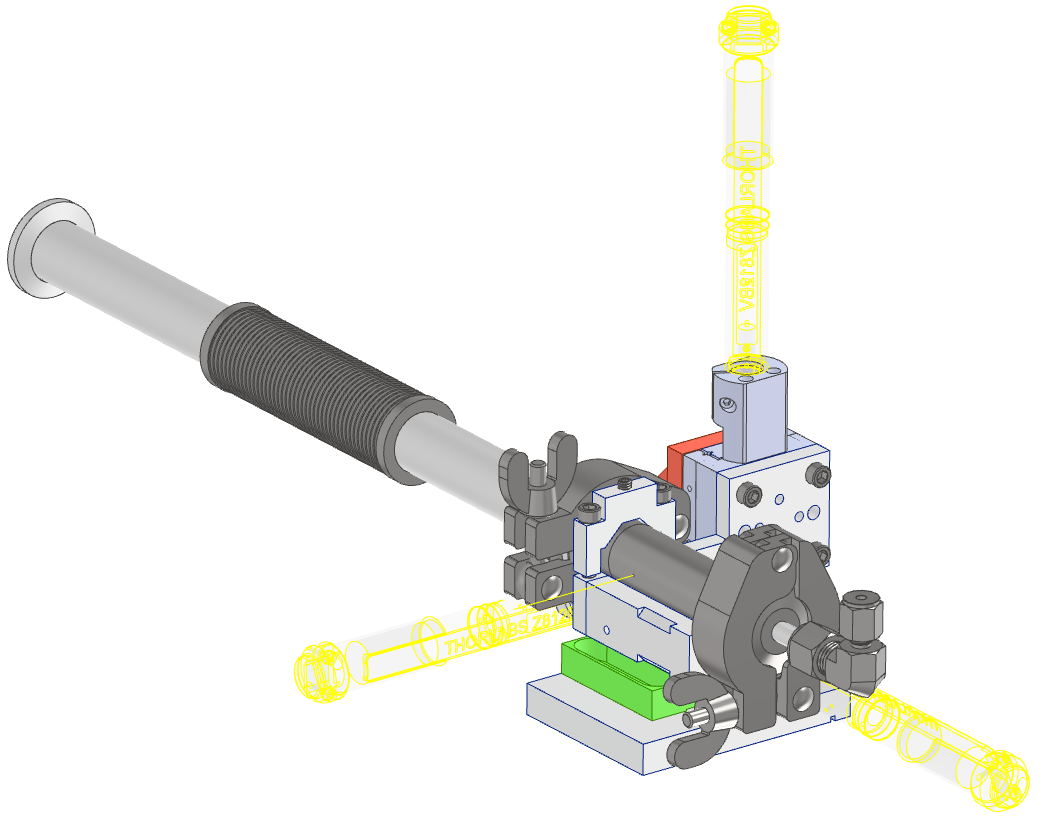
\includegraphics[width=0.9\textwidth]{figures/app1/HPC_on_stage2.png}
	\caption{The HPC with bracket installed on the XYZ translation stage, configured for the generation chamber. The hose clamp and gas supply tube is omitted from this drawing for clarity.}
	\label{fig:HPC_on_stage}
\end{figure}

\begin{figure}
	\centering
	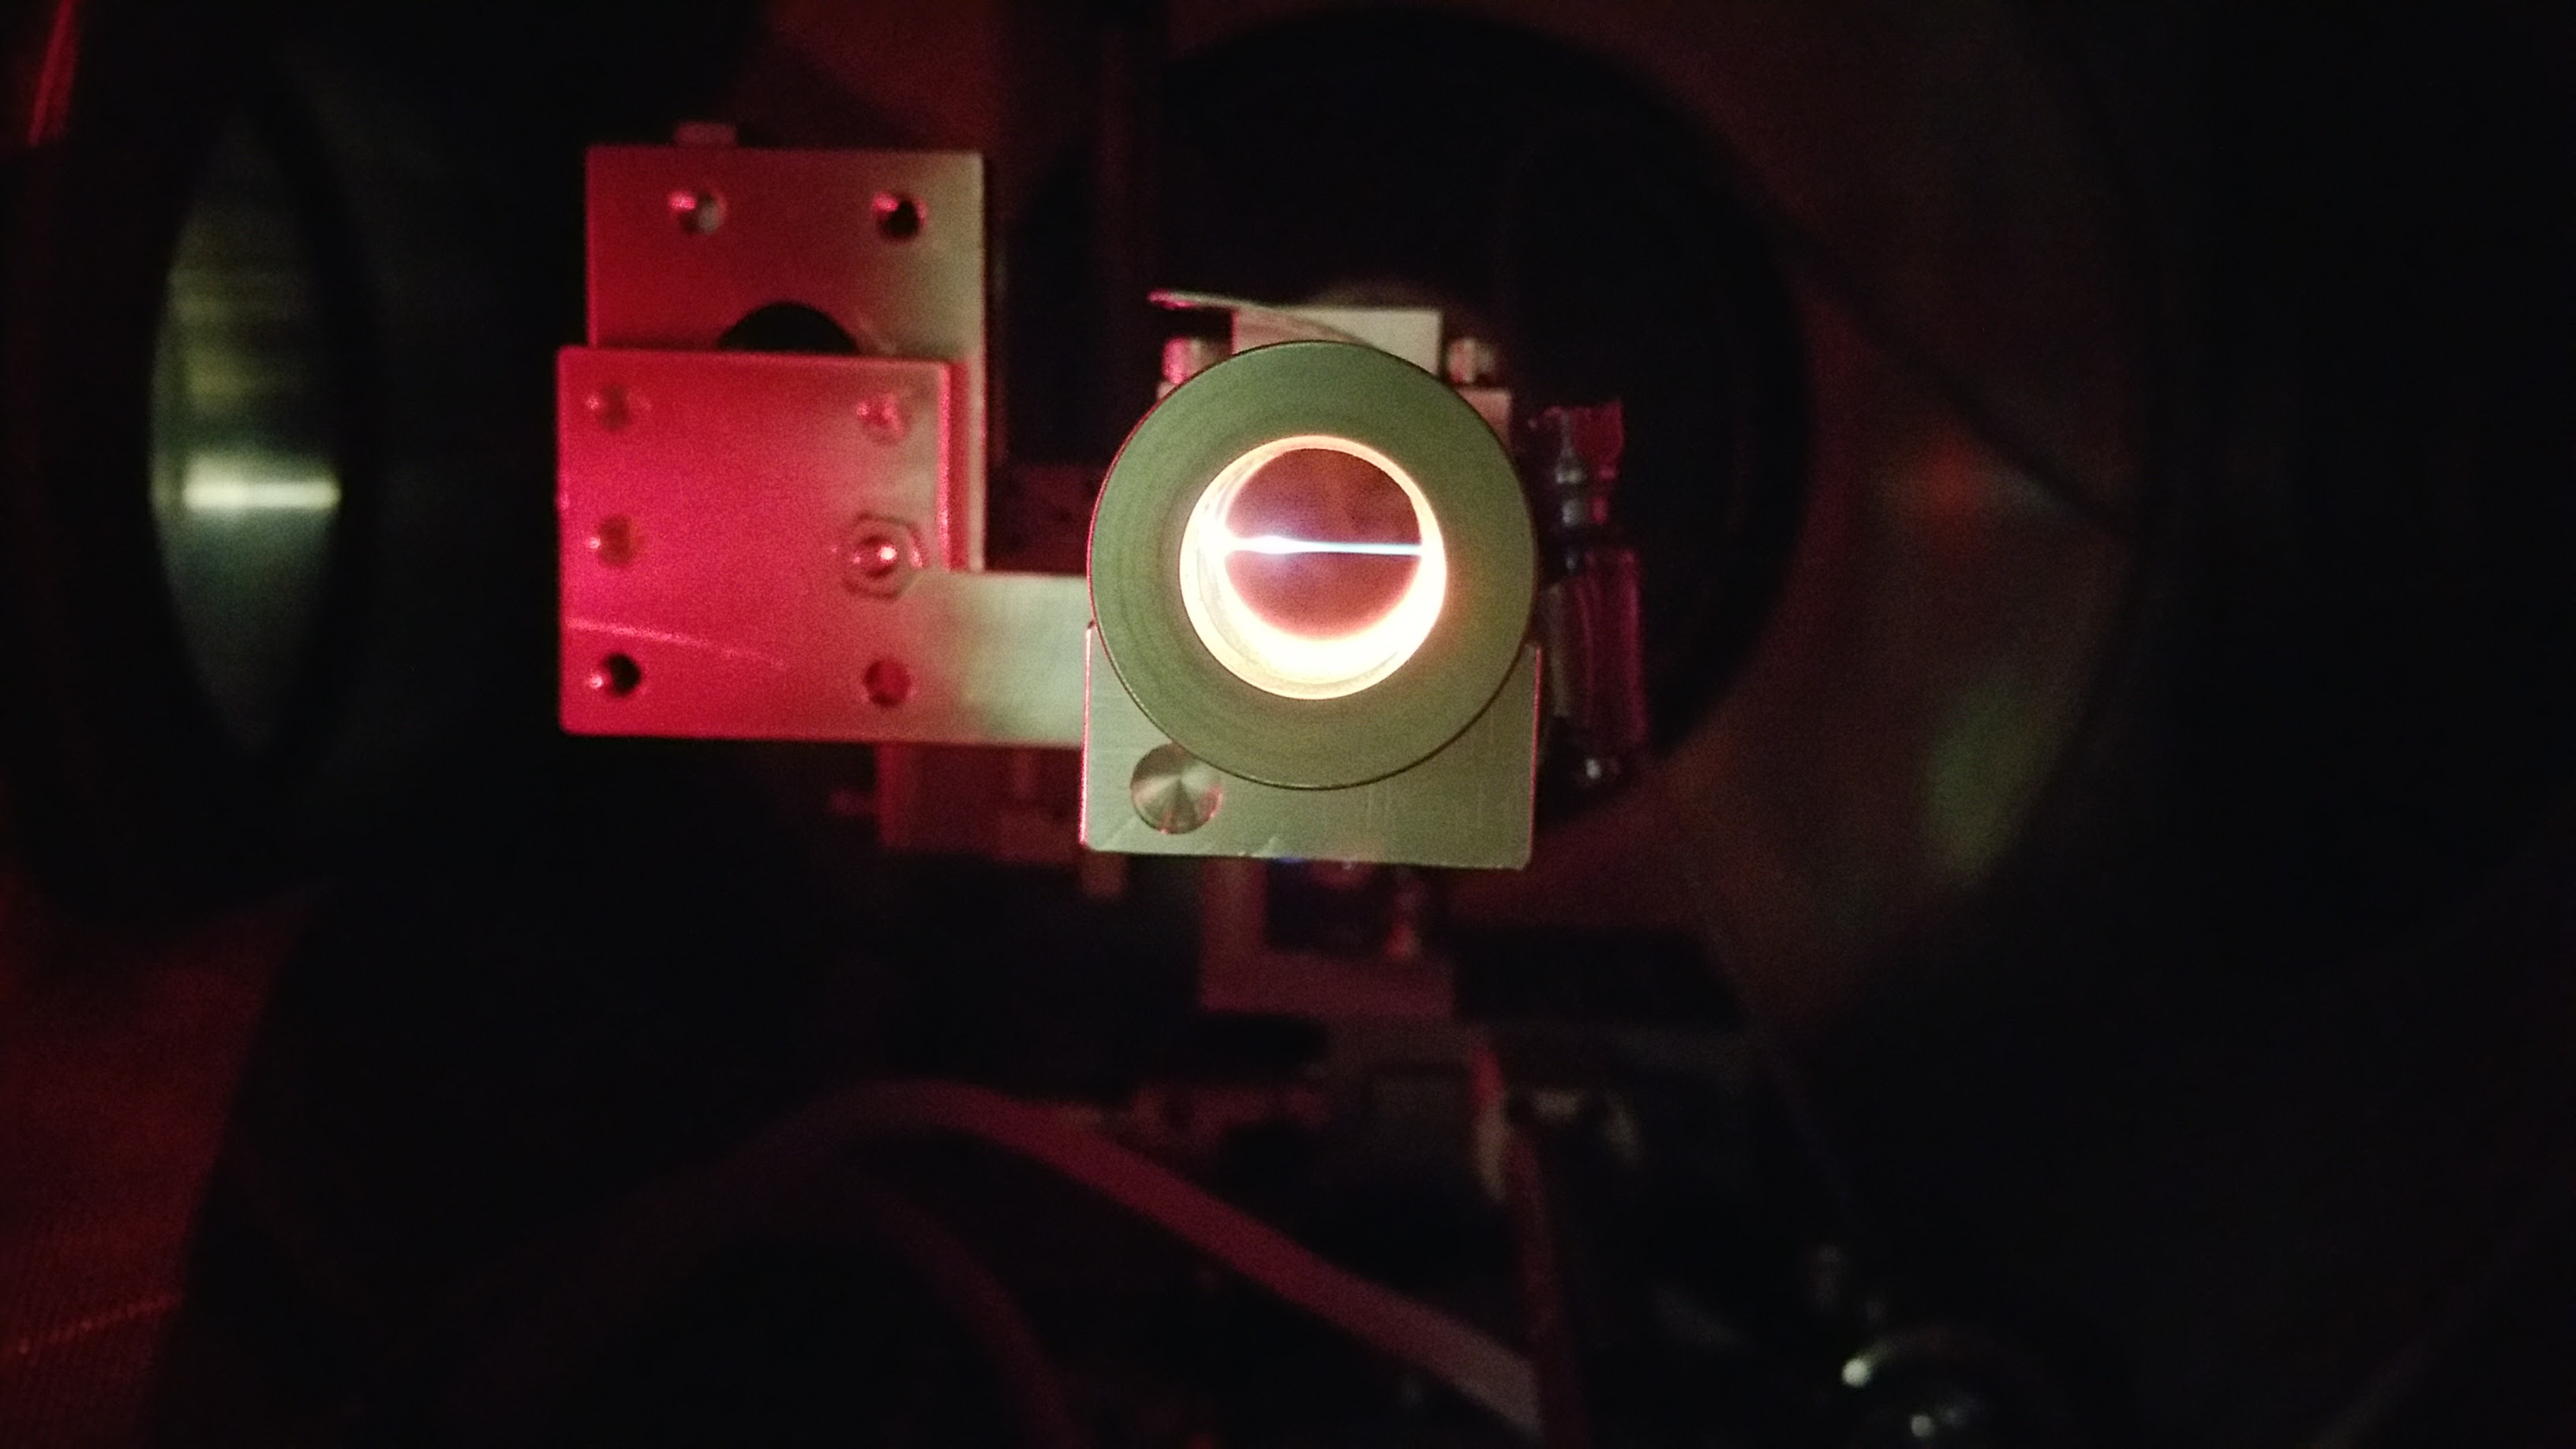
\includegraphics[width=0.75\textwidth]{figures/app1/HPC_outer_can_laser.jpg}
	\caption{Laser filament in the aligned outer pipe of the HPC. The inner pipe is not yet installed. Alignment of the outer pipe is done at very low intensities; after alignment the power was increased to create a filament for illustrative purposes only. This picture was taken in the target chamber during the initial testing of the HPC. The geometry of this chamber requires that the orientation of the mounting bracket is reversed compared to what is shown in Fig \ref{fig:HPC_on_stage}.}
	\label{fig:HPC_outer_can_laser}
\end{figure}

\begin{figure}
	\centering
	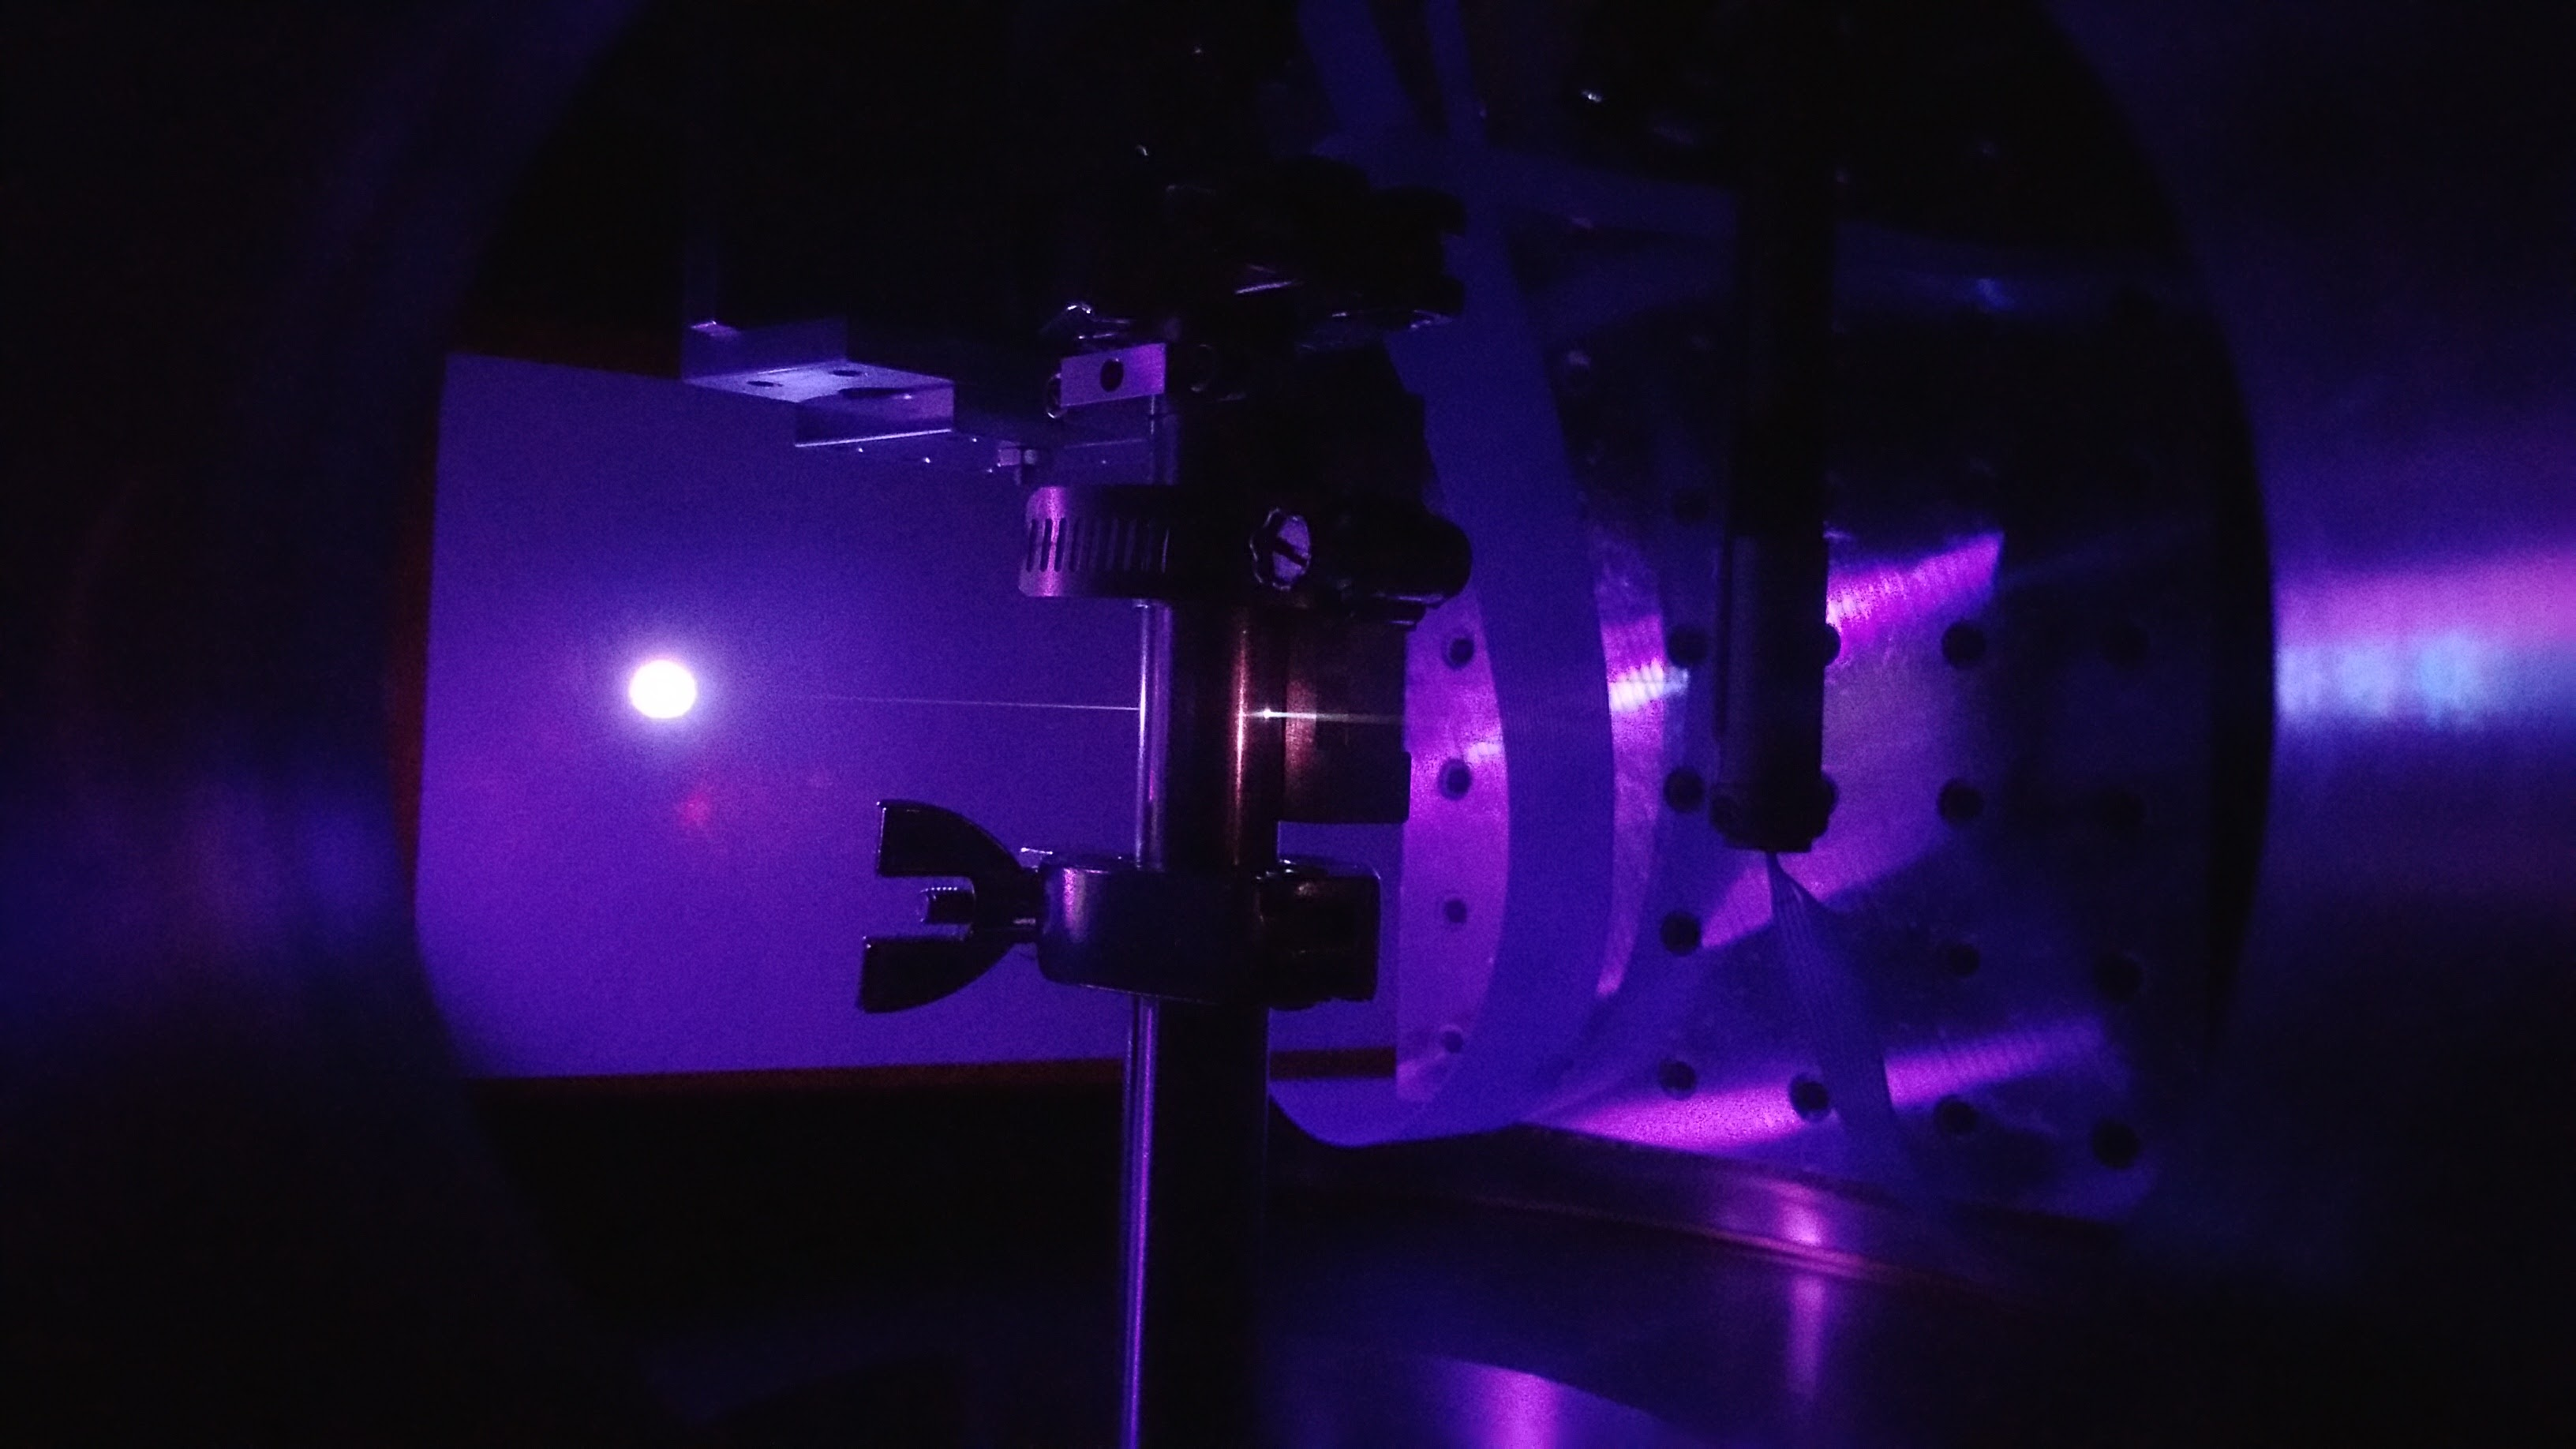
\includegraphics[angle=270, width=0.5\textwidth]{figures/app1/HPC_drilling.jpg}
	\caption{Laser drilling the inner pipe. A card blocks the laser after exiting the HPC. The HPC was pressurized with Ar gas to enhance the filament for illustrative purposes.}
	\label{fig:HPC_drilling}
\end{figure}

\subsection{Introduction}
\textit{main text: description of the HPC's design, pressure \& harmonic performance, pressure modeling, phase matching considerations. this section: how to install and actually use the HPC, how to machine or reorder certain parts.}

- focal length considerations. range of acceptable focal lengths. advantages of reflective vs transmissive focusing. possible schemes for shorter focal lengths. 

- space constraints of TABLe generation chamber limit the size of the XYZ stack. these are Newport 9066 1/2" travel stages, with 1" travel thorlabs motors (that's what we had, ideally you would use 1/2" motors). as a result, you can accidentally drive the motor more than the stage will allow. this will result in the motor falling out of the stage. in this case, you will have to immediately block the laser, vent the chamber, and reattach the motor. note: travel of all motors is from 0 to 14 mm.

- in-vacuum manipulation via the vacuum bellows (limits of motion, max pressure differential)

The ancillary vacuum hardware can be seen in Fig \ref{fig:HPC_outside_view}. A small oil-lubricated RV pump (not shown in this picture) provides differential pumping to the interior of the HPC. An inline Baratron diaphragm pressure sensor (effective range: 1 - 760 Torr) tracks the interior pressure of the edge-welded bellows. A manual gate valve is used to isolate the HPC from the RV pump when the additional pumping is not needed. Right angle KF fittings were used to route the HPC's vacuum line above the pump arm of the interferometer.


\subsection{Initial Installation and Alignment}
\label{app:initial-alignment-HPC}
First, a note about laser safety. The following alignment procedure should be done at the lowest possible laser power to minimize both accidental drilling of the HPC and the danger posed by stray light. Stray reflections or scatter from the many metallic surfaces of the HPC assembly pose a potential safety risk during alignment. The surface most likely to cause laser scatter is the front face of the outer pipe, which is roughened stainless steel located about 3/8" before the focus. The material's roughness and the negative radius of curvature of the incoming light make it unlikely that incident light will coherently focus to a point upon reflection. However, it is possible that the sidewall of the outer pipes's aperture could act as a focusing mirror. Additionally, the hose clamp or mounting bracket could coherently reflect light towards the user. The user is advised to strictly follow all laser safety protocols during this alignment procedure. Whenever possible, direct observation of the laser beam on the surfaces of the HPC should be avoided, instead a webcam should be used to view the interior of the generation chamber.

The initial installation of the HPC can be time consuming and tedious, but once installed it will retain its alignment for a period of weeks or months. The pointing into the cell should be done on a daily basis, but this is only slightly more complicated than what must be done with a free expansion gas jet.

Optically, the HPC cell consists of four pinhole apertures (diametrically opposed pinholes on both the inner and outer pipes) with the laser focus near the center of the inner pipe. The optical transmission of the HPC is therefore very sensitive to the relative alignment of these components, as well as the pointing of the laser into the HPC. To simplify the alignment, the two innermost holes are laser drilled \textit{in-situ} after the outer pipe has been aligned. To maintain the relative alignment of the inner \& outer apertures, the user should refrain from adjusting the inner pipe after the initial alignment is completed. Therefore, daily alignment of the HPC should be performed using only the in-vacuum motorized XYZ stages.

The first step of the HPC installation is installing the rough vacuum feedthrough flange. The TABLe's generation chamber uses a custom flange (a 4.5" CF blank with a KF16 half nipple welded to the air-side and a KF16 bulkhead groove \& tapped holes machined into the vacuum side). To accommodate the length of the in-vacuum bellows, we use a custom 10" CF to 4.5" CF reducing nipple (OAL = 4.25"), which acts as a spacer between the feedthrough flange and the KF16 flange on the HPC. Although it was absent from the original design, a spacer 4.5" CF flange (thickness = 0.68") between the feedthrough and the reducing full nipple is used to relax the compression in the bellows and allow for a larger range of motion. For convenience, the user should install the edge-welded bellows to the bulkhead flange before installing the flange on the chamber.

The supporting bracket for the HPC was designed to be interchangeable with the free gas nozzle's bracket. This design, shown in Fig. \ref{fig:HPC_on_stage}, allows the user to change the gas source type without disturbing the alignment of the XYZ stage to the optical axis. For completeness, we will assume that the XYZ stage has been misaligned or removed from the chamber. First, the user should align the laser to the interferometer so that the laser path in the generation chamber can be used as a reference. Then, the stage should be positioned in the chamber so that the focus is roughly in the center of the stage's motion. Finally, the stage's z-direction should made parallel to the optic axis. This can be done by tracking the position of the laser on a card mounted to the stage while moving the stage upstream and downstream of the focus. After clamping the stage to the breadboard, check that the alignment is still true before continuing to the next step.

The next step is to align the outer pipe of the high pressure cell by maximizing its light transmission. This is best done in two steps: first, coarse alignment is done visually at low power (insufficiently intense to laser drill the pipe), followed by fine adjustments using a power meter at moderate intensities (above the noise floor of the power meter). Note that accidentally drilling out the outer pipe will reduce its differential pumping performance. Given the chamber's small size, it is not practical to place a power meter in the generation chamber after the focus during the alignment procedure. Rather, it is preferable to divert the beam out of the vacuum system using the linear actuator \& silver mirror assembly located approximately 85 cm downstream of the focus.\footnote{Special thanks to Eric Moore for designing and installing this optomechanical component.} When inserted, the linear actuator intersects the beam path and redirects the beam out of the vacuum system through a window onto the upper deck of the optical table. The beam size can be reduced using a focusing lens onto the face of a power meter. Note that for most generation focusing conditions, the large beam size at the diverting mirror makes this beam path lossy. To accurately calculate the transmission through the HPC, it is necessary to measure the power immediately after the HPC in the generation chamber.

For the coarse alignment, the input beam intensity should be reduced using an upstream iris, to the point that it is barely visible near the focus. Since a tightened KF connection prevents rotation of the components, the alignment of the outer piper is done prior to making any KF connections. However, the KF clamps should be fitted on either end of the pipe to ensure that there is enough room to make the connections without disturbing the alignment once finished. The outer pipe should be placed in its cradle, with the aluminum \& hose clamps made snug around the pipe but not taut.\footnote{The HPC's XYZ assembly and bracket were designed for the TABLe generation chamber. If it is being installed elsewhere, the user should verify that the height is correct. When installed correctly, the bottom of the Z-motor range should correspond to the HPC lowered completely out of the way of the laser; the top of the range should correspond to the laser going through the center of the HPC, with about 1 mm to spare.} Transmission should be optimized by iteratively tuning the following parameters: (1) rotation of the pipe in the cradle, (2) height of the cradle using the vertical motor, and (3) horizontal (transverse) position of the assembly using both the horizontal motor and the position of the pipe in the cradle. For fine adjustment, the iris should be adjusted so that the power meter reads about 20-30 mW when measured after the linear actuator.\footnote{This power is appropriate for a 1kHz repetition rate and a generation focal length of 30 or 40 cm.} The clamps should be tightened so that movement of the pipe is possible, but difficult. The area around the power meter should be covered to prevent air currents from affecting the measurement. The transmitted power should be optimized using the same procedure as before.

Once the outer pipe is aligned, tighten all connections and connect the bellows to the outer pipe. Check that the alignment has not been changed by torquing these connections. Verify that the unattenuated laser beam can pass through the outer pipe without interference, as shown in Fig. \ref{fig:HPC_outer_can_laser}. If everything looks good, we can proceed to install the inner pipe.

First, attach the gas delivery feedthrough flange onto the HPC assembly without the inner pipe. Being mindful to not disturb the alignment of the outer pipe, check that the gas delivery tubing does not interfere with the laser path. Remove the gas delivery feedthrough flange, cut the inner pipe to length (OAL = 1.75"), and make the Swagelok connection between the inner pipe and the KF feedthrough. Make sure the inner pipe is normal to the flange's sealing surface, otherwise the laser will skim the sidewall of the inner pipe rather than go through the center. Install the gas delivery assembly onto the HPC assembly by tightening the KF clamp.

Laser drilling the inner pipe will sputter a significant amount of metal onto the inner surfaces of the chamber. Since the active drilling surface is on the upstream face of the pipe, most of the material will go upstream. Therefore, the laser window needs to be swapped out for a "sacrificial" window prior to drilling.\footnote{After drilling, the sacrificial window will be completely coated with a thin metal film. Most of the metal can be removed using methanol, but don't expect to be able to use the window for anything but laser drilling. Using a window with different optical properties (i.e., thickness or material), or no window at all, will change the pointing and effective focal length of the beam. It has been suggested that the laser window could be protected by placing a thin sheet of transparent plastic (Saran Wrap) between the window and the HPC, but we haven't tested this method.} Out of an abundance of caution, close the gate valve to the mirror chamber, retract the linear actuator \& silver mirror from the beam path, and block the generation chamber's vacuum aperture with a card.

Laser drilling should be done with the appropriate safety precautions: wearing laser goggles, notifying fellow labmates of your activity, and posting signs on the entrances to the lab. The user can cover up the chamber's flanges and set up a webcam to remotely monitor the laser drilling status to minimize the risk of inadvertent laser exposure.

At this point, the actual process of laser drilling is quite simple. There is no way to control the exact positioning of the inner pipe relative to the outer pipe, so there are no adjustments to make. Rather, the design relies on the mechanical alignment of the inner pipe relative to the outer pipe, which is ultimately set by the gas feedthrough weld, the Swagelok and the KF fitting. On the other hand, a used inner pipe cannot be reinstalled to the HPC once it is removed, since alignment is effectively impossible. To laser drill the pipe, simply let the unattenuated beam into the chamber and wait a few minutes until the laser emerges from the exit of the HPC. See Fig. \ref{fig:HPC_drilling}.

If you are planning on scanning the k-direction of the HPC during an experiment, you should do so now while you are set up for laser drilling. Similarly, if you are using a non-reflective (achromatic) focusing scheme and are planning on changing wavelengths during your experiment (which will change the effective focal length), you should step through the full range of wavelengths while drilling. Doing so will open up the apertures slightly, resulting in additional metal deposition on the sacrificial laser window.

After laser drilling is complete, reinstall the laser window and verify the HPC has retained its alignment.



\subsection{Alignment with the HPC Installed}

The daily pointing procedure, described in \ref{app:pointing-into-TABLE}, is largely unchanged by the presence of the HPC. However, there are some extra considerations that need to be made if the HPC is installed. The small apertures of the HPC and the non-linear nature of HHG demand high accuracy in the pointing into the cell, so small corrections to the positioning of the HPC have to be made after the daily pointing procedure is completed.

\subsubsection{Pointing into the Interferometer}
If the interferometer is already aligned, the presence of the HPC does not really complicate the daily procedure of the beamline. In this case, the user should block the laser into the generation chamber and align the pointing into the interferometer using the pump arm, as usual.\footnote{Failure to block the laser prior to changing the pointing may result in laser-drilling the HPC.} The procedure described in \ref{app:pointing-into-TABLE} is sufficiently accurate to get the laser through the HPC, but it won't necessarily yield optimized harmonics. Rather, the user may have to make small tweaks to the transverse position of the HPC. This can be done by optimizing the harmonic flux by making small (10 - 25 $\mu$m) steps using both the vertical and horizontal HPC motors while monitoring the harmonic yield using a fast camera exposure ($< 0.5$ s). In our experience, the optimal HPC position is typically within 50 $\mu$m of the previous day's position.

The HPC's apertures may no longer be circular if the HPC has been subjected to accidental laser drilling or significant laser drift. Non-circular apertures may result in a complex spatial profile of the harmonics, which can make the optimization of the harmonic yield difficult.

\subsubsection{Aligning the Interferometer}
If the interferometer needs to be realigned, then the HPC must be lowered out of the way of the laser. This is because the spatial mode of the IR is distorted by the HPC's apertures, which can introduce small shifts in the pointing of the IR after the HPC. Once the HPC is out of the way, the alignment procedure described in \ref{app:aligning-interferometer} can be followed without modification. Unless major changes were made to the interferometer, the angle of the HPC's apertures should remain aligned to the k-vector of the generation arm. In this case, the optimal position of the HPC can be found by maximizing the transmitted power of an the attenuated laser through the HPC, as described in the latter part of \ref{app:initial-alignment-HPC}. If major modifications were made to the interferometer, the user should consider aligning the HPC from scratch.


\subsection{Pump Down Procedure}



- pump down procedure

- generating and optimizing harmonics

- max internal pressure / pressure differential of the bellows tube

- max displacement of the tube

\subsection{Startup and Shutdown}


\section{Laser System Specifics}
importance of pointing \& laser performance for our experiments

\subsection{The Spitfire}
\subsubsection{Regular Maintenance}
- cleaning the stretcher

- increasing the pump laser currents

- changing the chiller fluid, desiccants, etc

\subsubsection{quirks and features}
- regen cavity tweaks

- photodiode problems

- software issues - bugs and troubleshooting

\subsection{Pointing Stabilization into the External Compressor}
- dietrich plots for pointing
\subsection{The Spitfire's External Compressor}
\subsubsection{external compressor alignment}
\subsubsection{cleaning the grating}

\subsection{The TOPAS-HE}
- aligning
- importance of power stability and pointing stability

\subsection{stability}
- boxing things up
- power stability throughout the day, people in the lab
- unstable harmonic yield from the HPC at high pressures
\section{The Shutter System}

\section{The Vacuum System}
- blower upgrade

- remote pressure sensing

- vacuum calculations for steady state pressure of beamline

\section{Best practices: data acquisition}

read-out noise from camera. (how noise scales)

\section{Steve's sections}
steve - grating alignment (which axes do what to harmonics?)

steve - 2-source / phase plate stuff, including calibration

steve - operating the cage and crank
%\chapter{Satellite stripe plot}

The satellite stripe plot can be made with data from any flight, however, this appendix shows how to create the plot using data from the \gls{anita}-2 and -3 flights (Figure~\ref{sat_stripe}). The plot is a two-dimensional histogram made with ROOT. The longitude of the \gls{anita} payload is in the vertical axis and the azimuthal reconstruction angle of events using their waveforms in \gls{lcp} is in the horizontal axis. The quantity in the horizontal axis, phi, is corrected for heading of the payload and calculated as shown in Equation~\ref{phi}. The color axis in the plot represents the number of events. Over-densities of events can be seen as stripes at certain longitudes. Each stripe is thought to be due to an individual group of satellites.

\begin{equation}
phi = fmod((phi_{LCP} - heading + 360),360)
\label{phi}
\end{equation}

\begin{figure}
\centering
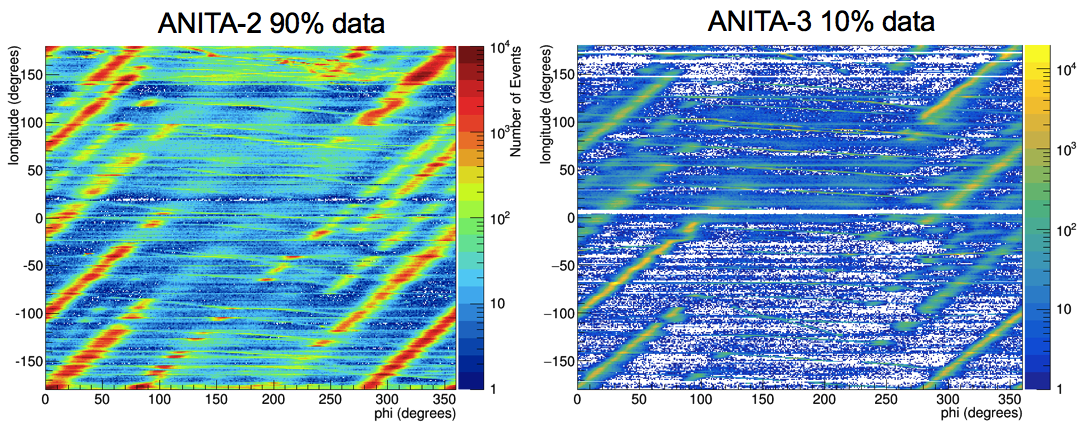
\includegraphics[width=1.0\textwidth]{figures/same_stripes.png}
\caption{Satellite stripe plots for the ANITA-2 and ANITA-3 flights.}
\label{sat_stripe}
\end{figure}

\section{Code for satellite stripe plot}

Example code used to make the satellite stripe plot for the \gls{anita}-3 and -2 flights are shown below. The \gls{anita}-3 code is a macro and runs independent of other \gls{anita} software. It needs to be run on Oakley as the \gls{anita}-3 data is located there. The \gls{anita}-2 code is meant to be compiled and run inside the \path{anita2code} directory of the binned analysis software which is located at:
\href{https://github.com/osu-particle-astrophysics/BinnedAnalysis}{https://github.com/osu-particle-astrophysics/BinnedAnalysis}. 

The code to make the \gls{anita}-3 satellite stripe plot is a macro called \path{plotLonPhi}. A macro is a piece of code in ROOT meant to serve only one function. Inside the macro, that function is written and the name of the macro is the same as the name of the function. 
In this particular macro, first I declare a TChain object. A TChain object is a collection of files containing TTrees. This is useful in \gls{anita} as you can add together the TTrees associated with data files of multiple runs into one object. To make the satellite stripe plot for \gls{anita}-3, we use the output files from runInterferometry.cxx of the \gls{anita}-3 binned analysis. These are saved as multiple ROOT files, one file per run. 

I used the 10\% data to make the \gls{anita}-3 plot. To use the 90\% data, change \path{sample_10} in the directory name to \path{sample_90}. Note that Draw, a member function of both TTree and TChain, is used. This allows one to make the plot without including the classes that data objects inherit from. The function Draw accesses what is inside the TTree directly without requiring a definition of the data type inside the tree. The plot can also be made in the traditional way of filling a histogram with entries from a TChain inside a for loop. 

The idea behind making the satellite stripe plot for \gls{anita}-2 is the same, however, the \gls{anita}-2 analysis software is unique. 
\gls{anita}-2 data is on Kingbee and that is where \path{anita2code} have been run and tested. The code to make the satellite stripe plot for \gls{anita}-2 is part of \path{oindreeskymap.cc} in \path{anita2code}. Note the \path{.h} files that must be included to run this code, especially \path{analysis_info_4pol.h}, which is a struct holding the necessary data variables. 


\par
\begin{verbbox}
/////////////////////FOR ANITA-3///////////////////////
void plotLonPhi();

void plotLonPhi()

{
  //Declare a TChain object (collection of files containing TTrees)
  TChain tchain("resultTree");
  
  //Add files containing data processed by interferometry
  tchain.Add("/fs/scratch/PAS0174/anita
  /2015_05_19/sample_10/geomFilter/analyzerResults_*.root");

  //Declare a TH2D object 
  //First argument is the name of the histogram
  //which is same as the variable name here 
  TH2D hlonPhi00("hlonPhi00","ANITA-3 10% Data LPol;
  phi (degrees);longitude (degrees)",360,0,360,360,-180,180);
  
  //Declare a TCanvas object 
  //which is needed to make a plot in ROOT
  TCanvas cL("cL","cL",900,800);
  
  //Use the Draw function to plot the histogram
  //TTree and TChain have this useful function Draw 
  //Draws and puts the histogram in the TH2D object you specified
  tchain.Draw("longitude:(fmod((peak[0][0].phi - heading + 360),360)) 
  >> hlonPhi00", "circPol == 1", "colz");
  //Set the color axis to log scale
  cL.SetLogz();
  //Save plot as a .png (or other chosen format)
  cL.SaveAs("LonPhiPeak00CPol1.png");
  //Save plot as .root as well for quick changes as needed
  cL.SaveAs("LonPhiPeak00CPol1.root");
  
}
\end{verbbox}
\fbox{\theverbbox}\par

\par
\begin{verbbox}
/////////////////////FOR ANITA-2///////////////////////
#include "analysis_info_4pol.h" //struct holding data variables 
using namespace std;
class MyCorrelator;
int main()
{
  char filename90[10000];
  char filename10[10000];
  sprintf(filename90,"/data/anita/btdailey/final_filter/
  90sample/geom_4pol_partial_0301/output*000.root");
  sprintf(filename10,"/data/anita/btdailey/final_filter/
  10sample/geom_4pol_partial_0301/output*.root");
  TChain tchain("analysis_info_4pol");
  tchain.Add(filename90);
  tchain.Add(filename10);
  
  //Create a pointer to instantiate struct 
  analysis_info_4pol *pol4_Ptr = NULL;
  tchain.SetBranchAddress("pol4_Ptr",&pol4_Ptr);
  
  //Note: R & L are switched in ANITA-2
  TH2D LonPhiR("LonPhiR","ANITA-2 100% Data After Quality Cuts;
  phi (degrees); longitude (degrees)", 360,0,360,360,-180,180);
  
  TCanvas cRmap("cRmap","cRmap",1000,800);
  tchain.Draw("pol4_Ptr->anitaLon:
  (fmod((pol4_Ptr->phiMap[3]-pol4_Ptr->heading+360),360)) 
  >> LonPhiR","","colz"); //R & L are switched in ANITA-2
  
  cRmap.SetLogz();
  cRmap.SaveAs("LonPhiR100pc.png");
  cRmap.SaveAs("LonPhiR100pc.root");
}
\end{verbbox}
\fbox{\theverbbox}

\end{document}
